% !TeX program = xelatex
\documentclass[12pt, twoside]{report}

% Packages
\usepackage{amsfonts,amsmath,amsthm}
\usepackage[utf8]{inputenc}
\usepackage[T1]{fontenc}
\usepackage{graphicx}
\usepackage{fontspec}
\usepackage[a4paper, width=150mm, top=25mm, bottom=25mm, bindingoffset=6mm]{geometry}
\usepackage{fancyhdr}
\usepackage[hidelinks]{hyperref}
\def\UrlBreaks{\do\/\do-}
\usepackage{nameref}
\usepackage[style=numeric, citestyle=authortitle]{biblatex}
\usepackage{algorithm,algcompatible}
\usepackage[noend]{algpseudocode}
\usepackage{algorithmicx}
\usepackage{float}
\usepackage{adjustbox}
\usepackage{url}
\usepackage[normalem]{ulem}
\useunder{\uline}{\ul}{}

%% Fonts
% main
\setmainfont{UT Sans}[
UprightFont=*-Regular,
BoldFont=*-Medium,
ItalicFont=*-Regular,
ItalicFeatures={FakeSlant=0.3},
BoldItalicFont=*-Medium,
BoldItalicFeatures={FakeSlant=0.1},
]
% algorithms
\newfontfamily{\algfont}{Courier}
\let\algorithmicOLD\algorithmic
\def\algorithmic{\algorithmicOLD\algfont}

% Header & Footer
\pagestyle{fancy}
\fancyhead{}
\fancyhead[LO,RE]{Manghiuc Teodor-Adrian \\ Informatică Aplicată}
\fancyhead[RO,LE]{Universitatea Transilvania \\ Facultatea de Matematică și Informatică}
\fancyfoot{}
\fancyfoot[LE,RO]{Pag. \thepage}
\renewcommand{\headrulewidth}{0.4pt}
\renewcommand{\footrulewidth}{0.4pt}
\renewcommand{\figurename}{Fig.}
\renewcommand{\chaptername}{Capitolul}
\renewcommand{\tablename}{Tabelul}
%\rhead{Manghiuc Teodor-Adrian \\ Informatică Aplicată}
%\lhead{Universitatea Transilvania \\ Facultatea de Matematică și Informatică}

% Disables paragraph indentation
\setlength{\parindent}{0pt}

% Graphics path
\graphicspath{ {Images} }

% Biblatex References
\addbibresource{references.bib}

% Algorithm comments
\renewcommand{\COMMENT}[2][.5\linewidth]{%
	\leavevmode\hfill\makebox[#1][l]{~#2}}

% General info
\title{Lucrare de licență}
\author{Manghiuc Teodor-Adrian}
\date{}

% Document
\begin{document}
	\begin{titlepage}
	\begin{center}
		
\includegraphics[width=240pt]{./Images/Logo/Logo-UT-MI-RGB-EN}
		\vspace*{48pt}\\
		\textbf{\LARGE Lucrare de licență}
		\vspace*{12pt}\\
		\LARGE FoodSpy\\
		\large Aplicație web pentru gestiunea aportului zilnic de calorii
		\vspace*{48pt}\\
		\begin{center}
			\large
			\begin{tabular}{ll}
				\textbf{Autor:}&Manghiuc Teodor-Adrian\\
				%\textbf{Mentor:}&\\
				\textbf{Coordonator:}&Monescu Vlad\\
			\end{tabular}
		\end{center}
		
		\vfill
		\large Brașov, România\\2020-2021
	\end{center}
\end{titlepage}
	
	\chapter*{Abstract}
	% !TeX root = ../FoodSpy.tex
% \section{Abstract}

Scopul lucrării este construirea unei soluții software moderne, care pune la dispoziție amatorilor în domeniul nutriției o interfață prietenoasă, intuitivă și ușor de folosit pentru menținerea unui jurnal al mâncărurilor consumate zilnic.
\\ \\
FoodSpy își propune să devină punctul de plecare către o aplicație mult mai complexă care poate ajunge să concureze cu soluțiile deja existente pe piață.

	
	\chapter*{Mențiuni}
	% !TeX root = ../FoodSpy.tex
% \section{Mentiuni}

Aș vrea să aduc mulțumiri domnului Lect. univ. dr. Vlad Monescu pentru ajutorul, îndrumarea și încurajările pe care le-am primit de la dânsul pe tot parcursul dezvoltării acestei lucrări.
\\ \\
Pentru sprijinul în configurarea adecvată a proiectului de Angular și pentru sprijinul învățării limbajului TypeScript, aș vrea să-i mulțumesc lui Gyulai Zoltán. Zoltán mi-a fost de mare ajutor în procesul de înțelegere al particularităților Angular.
\\ \\
Pentru sprijinul tehnic în dezvoltarea interfeței de programare aș vrea să le mulțumesc lui Alen Smailović și Florin Minecuța.
\\ \\
În cele din urmă aș vrea să aduc mulțumiri pentru încurajările, sfaturile și indicațiile primite de la mentorul meu, Ferenc Șipoș.
	
	\tableofcontents
	
	\chapter{Introducere}
	% !TeX root = ../FoodSpy.tex
% \section{Introducere}

\section{Motivarea alegerii temei}
FoodSpy este o aplicație web care își propune să îndeplinească un singur rol - acela de a permite amatorilor interesați de domeniul nutriției să mențină un jurnal al mâncărurilor consumate zi de zi.


\section{Soluții existente}
Eat \& Track
\\
O aplicație care ”este mai mult decât un simplu calculator de calorii”. Eat \& Track oferă în mod exclusiv alimente care se găsesc în magazinele din România, alături de rețete de mâncăruri și posibilitatea de a colabora cu specialiști în nutriție. De asemenea, permite urmărirea progresului spre obiectivele setate de utilizator. Un avantaj al aplicației este faptul că produsele pot fi scanate folosind camera telefonului și adăugate în jurnal; mai mult, scanând produsele, utilizatorii pot contribui și popula baza de date.\\
Eat \& Track oferă mult peste nevoile utilizatorului obișnuit, tocmai pentru a încearca să-l convertească într-un client al abonamentului PRO care promite atingerea mult mai ușoară a obiectivelor.


\section{Obiective propuse}
FoodSpy își propune să pună la dispoziția utilizatorilor o interfață prietenoasă, intuitivă și ușor de folosit.\\
FoodSpy este o aplicație care nu necesită instalare, ci o simplă conectare din orice browser, de pe orice dispozitiv.\\
FoodSpy își propune să ofere o soluție modernă la problema gestionării aportului zilnic de calorii, bazată pe infrastructura cloud.\\
FoodSpy nu colectează date despre utilizator, e-mail-ul și obiectivul caloric zilnic fiind folosite strict din motive funcționale.\\
	
	\chapter{Aplicații web - noțiuni teoretice}
	% !TeX root = ../FoodSpy.tex
% \section{Aplicații web - noțiuni teoretice}

\section{Arhitectura client-server}
Arhitectura client-server se referă la configurația de calculatoare în care server-ul găzduiește și administrează resursele și serviciile folositoare clientului. Mai multe calculatoare sunt legate la un server central printr-o rețea sau conexiune la internet pentru a putea partaja resursele de calcul.\\ \\
Clientul solicită o resursă de pe server printr-o conexiune la rețea, solicitarea fiind prelucrată și livrată înapoi clientului de către server. În această arhitectură, clientul este consumatorul, acesta utilizează serviciile oferite de server, și deci server-ul este producătorul. Serviciile oferite de către server sunt: stocarea datelor, partajarea datelor, accesul la aplicații sau accesul direct către resursele de calcul ale server-ului.\\ \\
Clientul execută următoarele operații: trimite solicitări către server, așteaptă și primește răspuns de la server și este activ, în sensul că este cel care inițiază operația de tranzacție între acesta și server.
\\ \\
Serverul este inițial pasiv, așteaptă o cerere de la client, verifică autorizarea, ascultă și este pregătit să răspundă solicitărilor clientului, iar când aceste solicitări sunt primite, le tratează, prelucrează și le trimite înapoi clientului sub forma unui răspuns.
\\ \\
Arhitectura client-server prezintă o serie de avantaje când vine vorba de persistența datelor:
\begin{itemize}
	\item avantajul centralizării tuturor datelor pe un singur server înseamnă că se pot simplifica operațiile de securizare ale datelor. De asemenea, operațiile de actualizare de date sau de software pot fi mai ușor de realizat
	\item avantajul de a fi accesibilă ușor, clientul putând să se conecteze la server de oriunde
	\item costurile comunicațiilor sunt reduse deoarece pe rețea circulă mai puține date pentru că o parte din operațiile executate de aplicație sunt efectuate la client
	\item configurarea serverului este mai ușoară fiindcă singura sarcina a server-ului este de a prelucra baza de date
\end{itemize}


\section{Hypertext Transfer Protocol}
HTTP este protocolul care permite accesarea de resurse, cum ar fi documente HTML. Reprezintă piatra de temelie pentru orice schimb de date pe web și este un protocol client-server. Browser-ul web este clientul și trimite cereri către server. Un document HTML complet este reconstituit din rezultatul mai multor sub-documente primite ca răspuns de la server. Sub-documentele pot fi bucățile de text care compun conținutul paginii, descrierea structurii paginii, imagini sau script-uri.
\\ \\
Clienții și server-ele comunică printr-un schimb de mesaje individuale și nu printr-un flux de date. Mesajele trimise de către client se numesc cereri (din engl. ”requests”), iar mesajele primite înapoi din partea server-ului se numesc răspunsuri (din engl. ”responses”).

\begin{figure}[!htb]
	\centering
	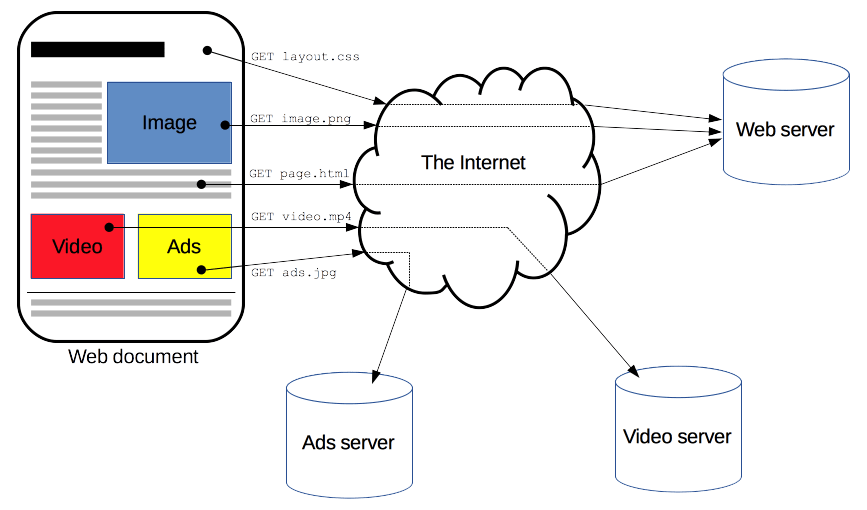
\includegraphics[width=1\textwidth]
	{../LaTeX/Images/http_fetch.PNG}
	\caption{Schimbul de mesaje între client și un server web}
	\label{fig:21}
\end{figure}

\subsection{Componentele unui sistem HTTP}
HTTP este un un protocol client-server, adică există o entitate care trimite cereri. Această entitate se numește ”user-agent” și este reprezentată de cele mai multe ori de un browser web, dar poate fi reprezentat și de un robot care menține un index pentru un motor de căutare.
\\ \\
Fiecare cerere se procesează în mod individual și întoarce un răspuns. Între browser și serverul care administrează cererile există nivelul de rețea și nivelul de transfer de date, format din router-e, modem-uri și altele. HTTP este deasupra acestor două nivele, deoarece face parte din nivelul de aplicație.
\\ \\
Pentru a afișa o pagină web, clientul trimite prima oară o cerere pentru aducerea documentului HTML care reprezintă pagina. Apoi, interpretează (din engl. ”parses”) documentul HTML și execută alte cereri. Aceste cereri corespund cu identificarea în fișier a script-urilor, opțiunilor de stilizare ale paginii (CSS) sau resursele media necesare, imagini și clipuri video. După ce toate aceste cereri au fost satisfăcute, browser-ul web pune toate părțile componente laolaltă și afișează pagina completă în fereastră.
\\ \\
O pagină web este un document ”hypertext”, adică poate conține legături către alte pagini web, accesibile la evenimentul de click al mouse-ului pe bucățile din text care reprezintă link-uri. Asta permite utilizatorilor să direcționeze clientul de pe o pagină pe alta și să navigheze pe web. Browser-ul este cel care interpretează aceste direcționări sub forma unor cereri HTTP de la care așteaptă răspuns. Răspunsul îl afișează utilizatorului sub forma unui mesaj clar.
\\ \\
La partea opusă a clientului stă server-ul, care așteaptă și administrează cererile primite. Un server nu este reprezentat neapărat de către o singură resursă de calcul. Folosind anumite soluții software, server-ul poate chiar partaja aceeași adresă IP cu alte server-e, folosind versiunea 1.1 a protocolului HTTP și antetul ”Host”. Antetul ”Host” specifică port-ul și gazda către care se trimite o cerere pentru a fi îndeplinită.

\subsection{Aspectele protocolului HTTP}
HTTP este gândit să fie simplu, extensibil și ”stateless”. ”Stateless” înseamnă că nu există o legătură între două cereri succesive, efectuate pe aceeași conexiune. Acest lucru ridică anumite probleme, deoarece un utilizator nu poate în mod coerent să interacționeze cu anumite pagini web, de exemplu, cu paginile web ale unui magazin online. Deși nucleul HTTP este ”stateless”, folosind cookie-uri HTTP se pot iniția așa numitele sesiuni ”stateful”. Folosind antetul unei cereri HTTP, cookie-urile se pot adăuga în antet, astfel încăt să permită creearea de sesiuni care partajează același context sau aceeași stare.

\subsection{Fluxul HTTP}
Se deschide o conexiune folosită pentru transportul cererii și al răspunsului.
Se trimite un mesaj HTTP, o cerere, după cum se poate observa în (Fig. \ref{fig:22}).

\begin{figure}[!htb]
	\centering
	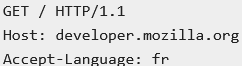
\includegraphics[width=0.5\textwidth]
	{../LaTeX/Images/http_message.PNG}
	\caption{Exemplu de mesaj HTTP}
	\label{fig:22}
\end{figure}

Răspunsul este ilustrat în (Fig. \ref{fig:23}). Acesta este citit de către client și interpretat.

\begin{figure}[!htb]
	\centering
	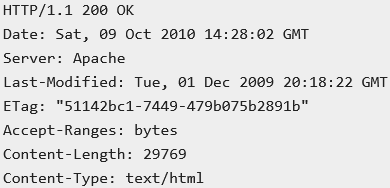
\includegraphics[width=0.8\textwidth]
	{../LaTeX/Images/http_response.PNG}
	\caption{Exemplu de răspuns HTTP}
	\label{fig:23}
\end{figure}

Pasul final este închiderea sau refolosirea conexiunii pentru alte cereri.

\subsection{Mesajele HTTP}
Există două tipuri de mesaje HTTP: ”request” și ”response”.
\\ \\
Un ”request” este compus din:
\begin{itemize}
  \item o metodă HTTP, de regulă ”GET” sau ”POST” care definește operația pe care clientul dorește să o efectueze
  \item calea către resursa de pe server dorită de client
  \item versiunea protocolului HTTP folosit
  \item anumite anteturi care oferă server-ului informații adiționale
  \item ”body”, dacă este vorba, de exemplu, de metoda ”POST” - acest ”body” poate conține o resursă trimisă de către client
\end{itemize}

Un exemplu de ”request” este ilustrat în (Fig. \ref{fig:24}).

\begin{figure}[!htb]
	\centering
	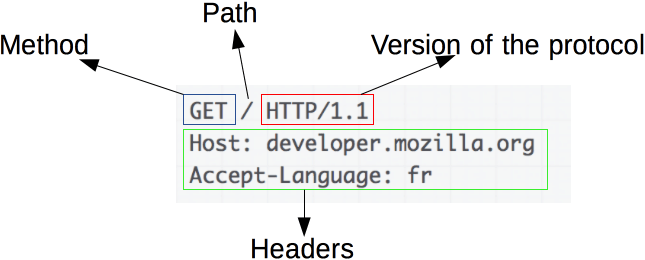
\includegraphics[width=0.7\textwidth]
	{../LaTeX/Images/http_request.PNG}
	\caption{Exemplu de ”request” HTTP}
	\label{fig:24}
\end{figure}

Un ”response” este compus din:
\begin{itemize}
  \item ”status code” care indică faptul că cererea a fost îndeplinită sau nu
  \item ”status message” care descrie pe scurt ”status code”
  \item versiunea protocolului HTTP
  \item anteturi
  \item ”body”
\end{itemize}

Un exemplu de ”response” este ilustrat în (Fig. \ref{fig:25}).

\begin{figure}[!htb]
	\centering
	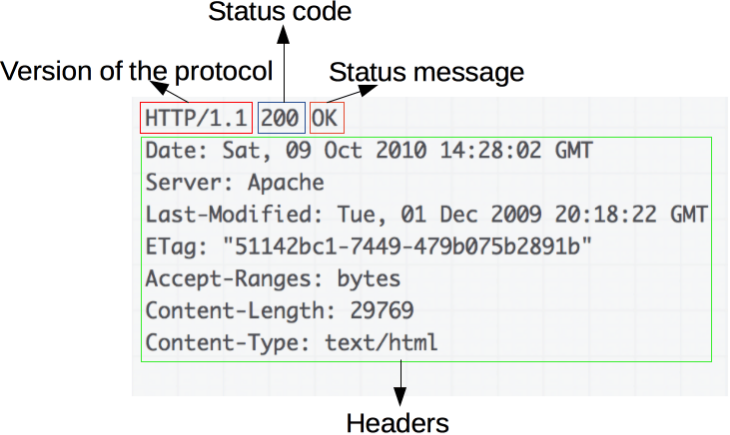
\includegraphics[width=0.7\textwidth]
	{../LaTeX/Images/http_response-ex.PNG}
	\caption{Exemplu de ”response” HTTP}
	\label{fig:25}
\end{figure}


\section{Aplicație web vs. site web}
Deși se accesează în același fel și arată la fel, o aplicație web nu este un website.\\
O aplicație web este construită cu scopul de a interacționa cu utilizatorul, în timp ce un website doar servește conținut static, conținut care nu poate fi afectat de către vizitator.
\\ \\
Website-ul este structurat pe mai multe pagini care au adrese web diferite și care indică resurse web diferite, în timp ce, de regulă, o aplicație web ”rescrie” în mod dinamic pagina curentă pe care se află utilizatorul; această ”rescriere” stă la baza așa numitelor ”single-page application”.
\\ \\
Pentru a putea interacționa cu aplicația web, un utilizator trebuie autentificat și autorizat \footnote{Dacă luăm un exemplu cu un club, prin autentificare se înțelege procesul de identificare a vârstei unui petrecăreț, pe baza unui buletin, în vreme ce prin autorizare se înțelege acordarea unor privilegii speciale acestui petrecăreț, accesul în zona VIP, în zona DJ-ului, și așa mai departe.}, în vreme ce vizitatorul unui website poate cel mult să se înscrie pe o listă de corespondență de unde poate primi notificări din partea administratorul website-ului.
\\ \\
Un website este un mod de afișare structurată a informației. Este un produs complet, accesibil printr-un browser web, nu necesită compilare, doar actualizarea structurii și informației, acolo unde este cazul, fără nevoia de implementare (din engl. ”deployment”).
\\ \\
O aplicație web este o soluție software sau un program, accesibil printr-un browser web. Spre deosebire de programele desktop, aplicația web este valabilă pe orice platformă deoarece sistemele de operare desktop suportă majoritatea browser-elor web moderne. De asemenea, pe sistemele de operare mobile nu este necesară aprobarea într-un magazin de aplicații (App Store sau Google Play) pentru a fi folosite pe aceste dispozitive. Aplicațiile web sunt mai ușor de întreținut deoarece folosesc același cod-sursă pentru toate platformele și mai mult decât atât, nu este necesară actualizarea lor de către utilizatori, cum este cazul aplicațiilor mobile.
\\ \\
Aplicația web are avantajul scalabilității și găzduirii în cloud. Poate fi folosită pe orice platformă, este modulară și suportă testarea acesteia folosind teste automate.


\section{REST API}
Acronimul REST vine de la ”representational state transfer” și este un stil arhitectural menit pentru construirea de aplicații web scalabile.
O interfață de programare (din engl. ”API”) REST are caracter ”RESTful” dacă se conformează constrângerilor impuse de stilul arhitectural REST.
\\ \\
Pentru a implementa un asemenea API, există câteva cerințe care trebuie îndeplinite și anume:

\begin{itemize}
  \item implementarea unei arhitecturi client-server compusă din clienți, server-e și resurse și folosirea protocolului HTTP pentru administrarea cererilor și răspunsurilor. Clientul trimite o cerere pe care server-ul o poate respinge sau o poate îndeplini prin oferirea unui răspuns adecvat.
  \item comunicare ”stateless” între client și server, astfel încât nicio informație de la client nu este stocată între mai multe cereri succesive, iar cererile sunt tratate în mod individual, separat și neconectat. Clientul și server-ul sunt prinși într-o secvență cerere-răspuns, în care clientul inițiază o cerere, iar server-ul răspunde. La cererile ulterioare, server-ul nu cunoaște răspunsurile pe care l-a oferit anterior.
  \item posibilitatea stocării în cache pentru facilitarea comunicării dintre client și server. Cererile inițiate de client au caracter independent. La momentul repetării uneia dintre aceste cereri, răspunsul este stocat în cache la nivelul clientului. Când clientul repetă o cerere, aceasta nu mai ajunge până la server, ci este oferit răspunsul direct din cache.
  \item folosirea unei interfețe uniforme între componentele arhitecturii astfel încât informația poate fi transferată sub o formă standard:
	\begin{itemize}
		\item resursele cerute de client sunt identificabile și separate de reprezentările oferite înapoi clientului
		\item resursele pot fi manipulate de către client via reprezentările oferite, deoarece acestea conțin suficiente informații astfel încât să permită manipularea lor
		\item mesajele oferite alături de răspunsul de la server trebuie să fie ușor de interpretat, astfel încât clientul să le poată procesa
	\end{itemize}
  \item un sistem stratificat care organizează fiecare tip de server responsabil pentru îndeplinirea cererilor, în ierarhii, invizibile clientului. Asta face posibilă implementarea unui strat adițional, numit ”middleware” care stă între client și server. Clientul poate interacționa cu stratul ”middleware”, dar clientul nu trebuie să recunoască prezența acestuia.
  \item opțional, se poate implementa ”code-on-demand”, prin care se permite trimiterea codului executabil de la server către client, la cerere, extinzând astfel funcționalitatea API-ului
\end{itemize}

REST este un set de constrângeri arhitecturale, nu un protocol sau un standard. Dezvoltatorii de interfețe de programare ”RESTful” pot deci să implementeze acest stil arhitectural în mai multe feluri, dar respectând cerințele.
\\ \\
REST constituie o cale de acces către resursele care sunt stocate într-un anume mediu. De exemplu, un server poate stoca o colecție de documente și imagini, iar fiecare document și fiecare imagine reprezintă o astfel de resursă. REST definește un serviciu care spune cum ar trebui să fie implementat accesul către aceste resurse.
\\ \\
Definiție pentru o resursă web. O aplicație web poate fi folosită, de exemplu, pentru accesul la datele despre angajații unei firme. Fiecărui angajat îi corespunde o înregistrare în baza de date. Dacă URL-ul pentru aplicația web este ”http://demo.a3drian.com”, la datele despre unul dintre angajați se ajunge printr-o cerere către URL-ul\\”http://demo.a3drian.com/employee/1”. La momentul îndeplinirii acestei cereri, se aduc datele despre angajatul care are ”ID”-ul ”1”.
\\ \\
Definiție pentru metodele HTTP. Aceste metode descriu felul în care clientul dorește să interacționeze cu o resursă. Principalele metode sunt:
\begin{itemize}
  \item GET
  \item POST
  \item DELETE
  \item PUT
  \item PATCH
\end{itemize}

Metodele sunt explicate în detaliu în (Tabelul \ref{fig:26}).

\begin{table}[]
\centering
\resizebox{\textwidth}{!}{%
\begin{tabular}{lll}
URL          & metodă & funcționalitate                                                             \\
\hline
employees/10 & GET    & aduce datele despre un singur angajat (o singură resursă)                   \\
employees    & GET    & întoarce întreaga listă de angajați (toate resursele)                       \\
employees    & POST   & creează o nouă resursă cu datele primite în corpul (”body”) cererii         \\
employees/10 & DELETE & șterge resursa cu ID-ul ”10”                                                \\
employees/10 & PUT    & înlocuiește conținutul unei resurse cu datele primite în cerere             \\
employees/10 & PATCH  & înlocuiește doar o parte a conținutului unei resurse cu datele primite în cerere
\end{tabular}%
}
\caption{Descrierea în detaliu a metodelor HTTP}
\label{fig:26}
\end{table}

Definiție pentru anteturi. Anteturile sunt folosite pentru a trimite server-ului informații adiționale legate de cerere. Spre exemplu, ”Content-Type: text/html; charset=UTF-8” este antetul care impune server-ului să răspundă cu o resursă în format ”text/html” și având setul de caractere ”UTF-8”. Un alt exemplu este ”Authorization” - antetul care conține credențialele necesare clientului pentru procesul de autentificare.
\\ \\
Definiție pentru ”body”-ul cererii. O cerere poate să conțină informații sub formă de date. De regulă, datele sunt trimise împreună cu o cerere atunci când se execută metoda ”POST”. Metoda ”POST” comunică server-ului faptul că dorește să adauge o nouă resursă. Astfel, în corpul (”body”) cererii sunt conținute datele pe care server-ul le folosește pentru adăugarea resursei noi.
\\ \\
Definiție pentru ”body”-ul răspunsului. Acesta reprezintă corpul principal al răspunsului. Referindu-ne la exemplul de mai sus, când URL-ul pentru aplicația web era ”http://demo.a3drian.com”, atunci când se face o cerere ”GET” la URL-ul\\”http://demo.a3drian.com/employee/1” server-ul poate întoarce datele despre angajatul cu ”ID”-ul ”1” sub formă de JSON sau sub formă de XML.
\\ \\
Definiție pentru ”status code”. Reprezintă o colecție de numere întregi și constituie codurile care se returnează alături de răspunsul venit de la server. ”200” este codul care se atașează răspunsului, atunci când cererea clientului a fost îndeplinită cu succes. ”404” este folosit în momentul în care resursa cerută de client nu a fost găsită pe server, iar ”504” este codul rezultat atunci când server-ul este offline. Alături de aceste coduri, server-ul trimite și un scurt mesaj. Lângă ”200” se atașează ”OK”, lângă ”404” server-ul întoarce mesajul ”Not found”, iar lângă ”504” mesajul returnat este ”Gateway timeout”.
	
	\chapter{Limbaje de programare}
	% !TeX root = ../FoodSpy.tex
% \section{Limbaje de programare}

\section{JavaScript / TypeScript}
JavaScript este un limbaj de programare care permite implementarea unor funcționalități complexe în paginile web. Câteva dintre aceste funcționalități sunt actualizarea conținutului paginilor web în mod dinamic, animarea de grafice 2D sau 3D și afișarea hărților interactive. Alături de HTML și CSS, JavaScript este unul dintre tehnologiile web standard.
\\ \\
JavaScript este un limbaj multi-platformă, poate fi folosit pe partea de client, dar și pe partea de server, este ușor de învățat și este dinamic și flexibil. Această dinamicitate este însă și unul din dezavantajele limbajului. De exemplu, JavaScript pune la dispoziție variabile primitive de tip ”string” sau ”number”, dar pentru că nu este necesară compilarea codului, nu se verifică folosirea corectă a acestor variabile, programatorul putând folosi o variabilă ”title” pentru a reține un ”string” (Fig. \ref{fig:31}), dar care mai târziu poate va fi suprascrisă și se poate reține (în variabilă) un ”number”, fără niciun fel de avertizare din partea mediului de programare, putând conduce la bug-uri și la comportamente neprevăzute.

\begin{figure}[!htb]
	\centering
	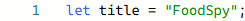
\includegraphics
	{../LaTeX/Images/ts_title-1.PNG}
	\caption{Definirea variabilei ”title”}
	\label{fig:31}
\end{figure}

Aici intervine TypeScript, un superset al limbajului JavaScript ce adaugă ”siguranța de tip” necesară pentru evitarea situațiilor neplăcute precum este cea descrisă mai sus. TypeScript încurajează scrierea codului în stil declarativ, asemănător limbajelor C\# sau Java prin facilități ca interfețe, clase și inferența de tip a variabilelor.
\\ \\
Este necesară compilarea codului scris în limbaj TypeScript, dar acest lucru poate fi văzut ca un avantaj pentru că mediul de programare poate astfel scoate în evidență comportamentul neașteptat al codului și prin urmare poate duce la detecția mult mai rapidă a bug-urilor. Referindu-ne la situația neplăcută descrisă mai sus, dacă variabila ”title” ar fi adnotată cu tipul ”string”, atunci nu va putea fi suprascrisă de o valoare pretabilă unei variabile de tip ”number”.
\newline

\begin{figure}[!htb]
	\centering
	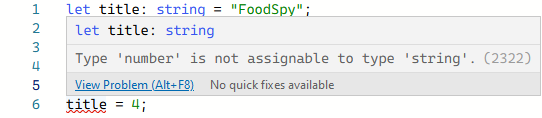
\includegraphics
	{../LaTeX/Images/ts_title-2.PNG}
	\caption{Adnotarea previne suprascrierea variabilei ”title”}
	\label{fig:32}
\end{figure}

TypeScript vine în ajutorul programatorilor care sunt deja obișnuiți cu limbaje de programare cu stil declarativ și propune astfel o alternativă față de JavaScript care nu oferă niciun suport pentru ”siguranța de tip”.
\\ \\
Deși o mai bună înțelegere a limbajului JavaScript este recomandată, TypeScript se poate învăța și folosi în mod independent, fără a cunoaște toate dedesubturile JavaScript. Mai mult, un bonus pentru programatorii cu experiență în C\# este faptul că autorul limbajului TypeScript este arhitectul limbajului C\#, deci, din punct de vedere sintactic, TypeScript și C\# împărtășesc multe similitudini.

\begin{figure}[htbp]
	\centering
	%\hspace*{-2cm}
	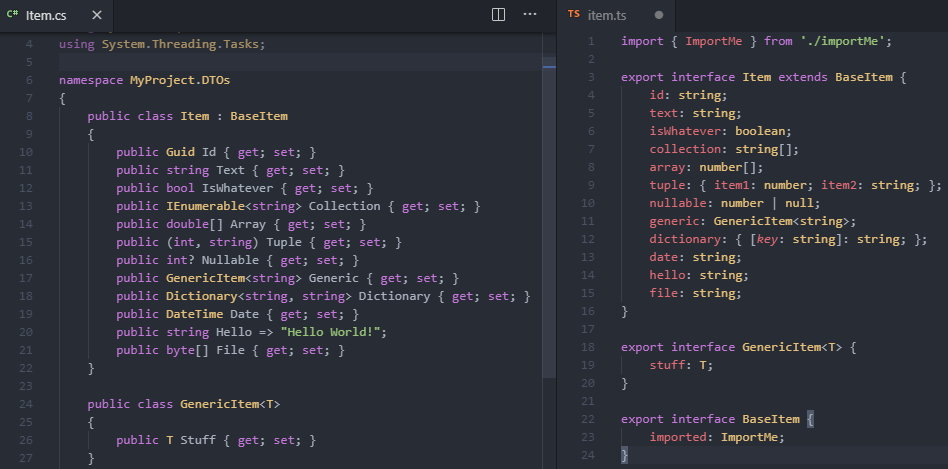
\includegraphics[width=1\textwidth]
	{../LaTeX/Images/ts_similar-3.PNG}
	\caption{Asemănări între C\# și TypeScript}
	\label{fig:33}
\end{figure}

Față de JavaScript, TypeScript întinde o plasă de siguranță care poate prinde defectele de programare introduse prin modificări majore ale codului. TypeScript nu va înlătura necesitatea depanării programelor, dar ”siguranța de tip” va ajuta fără echivoc la detectarea din timp ale defectelor. Mai mult, TypeScript beneficiază de sugestii și avertizări din partea mediului de programare încă de la compile-time, în timp ce erorile în JavaScript pot fi descoperite abia la run-time.
\\ \\
Printre alte avantaje ale TypeScript includem și posibilitatea re-factorizării într-un mod mai sigur deoarece se cunoaște codul la nivel semantic și capabilitățile TypeScript care permit construirea aplicațiilor de mărime foarte mare, în completă antiteză cu JavaScript care a fost gândit ca un limbaj folosit strict pentru modificarea dinamică a paginilor web.


\section{C\#}
C\# este un limbaj de programare orientat pe obiect, simplu, dar puternic și este gândit pentru dezvoltarea de aplicații pe platforma .NET Framework. Moștenește părțile bune ale limbajului C++ și Visual Basic, dar fără anumite inconsistențe \footnote{O astfel de inconsistență în C++ este accesul la un element dintr-un ”std::vector”. În C++ se poate folosi operatorul ”[]” pentru a ajunge la elemente care nu sunt de fapt elementele ale vectorului, ci sunt bucăți de informație conținute la adresele de memorie adiacente memoriei alocate vectorului. Deoarece nu se face niciun fel de verificare a indicelui elementului pe care încercăm să-l accesăm, operatorul ”[]” va întoarce ceea ce se află la locația de memorie vecină memoriei alocate vectorului.} și anacronisme ceea ce duc la un limbaj mai logic și mai puțin complicat.
La fel cum pentru o variabilă, simbolul ”++” înseamnă incrementarea cu 1 după ce variabila a fost evaluată, pentru C\#, simbolul ”\#” semnifică o incrementare a limbajului C++.
\\ \\
Prima versiune a apărut în 2001. Odată cu versiunea 2.0 au apărut lucrul cu generice, iteratori și metode anonime. În versiunea 3.0 au debutat metodele de extensie, expresiile lambda și cel mai important, LINQ sau Language-INtegrated Query. Versiunea 5.0 a venit cu suport nativ pentru operațiile asincron prin introducerea operatorului ”await” și modificatorului de funcție ”async”.
\\ \\
%\label{cgenerics}
Lucrul cu clase și metode generice reprezintă un concept care face posibilă proiectarea de clase și metode ale căror tipuri se cunoaște doar la momentul declarării sau instanțierii. Acest concept combină reutilizarea codului, ”siguranța de tip” și eficiența într-un mod în care nu este posibil prin proiectarea specifică.
\\ \\
”GenericList” din (Fig. \ref{fig:34}) este un exemplu de clasă generică care modelează o listă simplu înlănțuită capabilă să memoreze obiecte de tip ”Node” de orice tip, inclusiv ”int”, ”double” sau ”string”.

\begin{figure}[!htb]
	\centering
	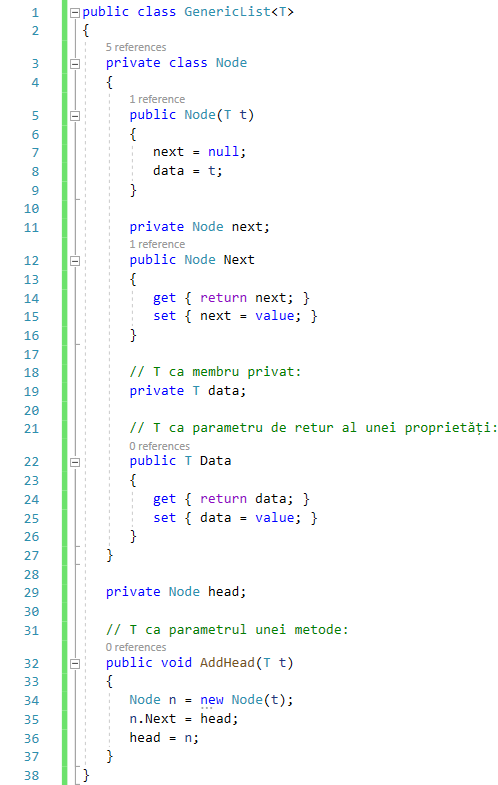
\includegraphics[width=0.8\textwidth]
	{../LaTeX/Images/csharp_generics.PNG}
	\caption{Exemplu de clasă generică}
	\label{fig:34}
\end{figure}

Parametrul de tip ”T” ia locul declarării tipului explicit și este folosit ca parametru în metoda ”AddHead(T t)”, ca parametru de retur al proprietății ”Data” și ca tip de membru privat, cum este cazul membrului ”T data”. La momentul instanțierii clasei ”GenericList<T>”, fiecare apariție a lui ”T” va fi înlocuită de tipul specificat între ”<>”.
Se pot crea interfețe, clase, metode, evenimente și delegați generici.
\\ \\
%\label{cextmeth}
Metodele de extensie sunt o funcționalitate a limbajului C\# care permit adăugarea de metode tipurilor deja existente. Metodele de extensie sunt metode statice care sunt apelate ca și cum ar fi membre ale clasei, cum este de exemplu metoda ”ToString()”, membră a clasei ”Object”.
\\ \\
O metodă de extensie are cel puțin un parametru, ”this” care reprezintă obiectul curent peste care operează metoda. Din cauza aceasta, când se apelează o metodă de extensie de către un obiect, obiectul nu trebuie trimis ca parametru.
”WordCount” din (Fig. \ref{fig:35}) este o metodă de extensie care numără caracterele dintr-un obiect de tip ”string”. Se observă că ”WordCount” este definită pentru obiecte din clasa ”System.String” deoarece parametrul ”str” este prefixat de ”this string”.

\begin{figure}[!htb]
	\centering
	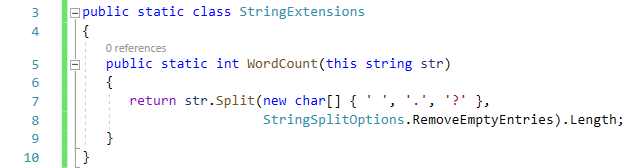
\includegraphics
	{../LaTeX/Images/csharp_extension-1.PNG}
	\caption{Exemplu de metodă de extensie}
	\label{fig:35}
\end{figure}

Apelul metodei de extensie se poate observa în (Fig. \ref{fig:36}).

\begin{figure}[!htb]
	\centering
	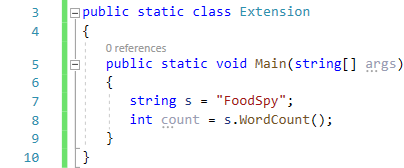
\includegraphics
	{../LaTeX/Images/csharp_extension-2.PNG}
	\caption{Apelul unei metode de extensie}
	\label{fig:36}
\end{figure}

%\label{clinq}
O definiție simplistă pentru LINQ este următoarea: modalitatea prin care se poate interoga o bază de date folosind un limbaj de interogare apropiat de SQL, dar care este compilat în interiorul unei aplicații care rulează pe platforma .NET.
Prin ”bază de date” se înțelege un spectru larg de surse de date, printre care baze de date SQL, baze de date ”in-memory” sau reprezentări XML.
\\ \\
LINQ permite scrierea unei interogări sub forma unei structuri SQL, după cum se poate observa în (Fig. \ref{fig:37}). Această structură are avantajul că variabila ”name” este ”scoped”, adică nu trebuie definită din nou pentru fiecare clauză din interogare.

\begin{figure}[!htb]
	\centering
	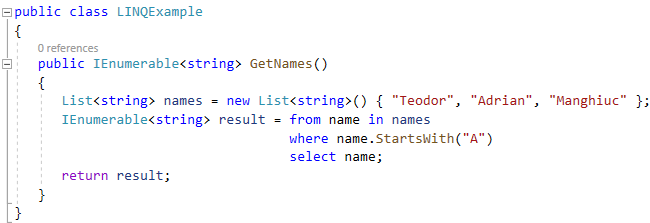
\includegraphics
	{../LaTeX/Images/csharp_linq-1.PNG}
	\caption{Exemplu de interogare LINQ}
	\label{fig:37}
\end{figure}

Un alt avantaj este claritatea originii variabilei ”name” - chiar din primul rând ("from name in names") se distinge faptul că ”name” provine din sursa de date ”names”, spre deosebire de interogarea SQL clasică, unde clauza ”from” ar fi fost declarată ultima.

LINQ nu ar fi fost un concept realizabil dacă nu s-ar fi implementat în prealabil funcționalități precum metodele de extensie, tipurile anonime \footnote{List<string> names = new List<string>() \{ "Teodor", "Adrian", "Manghiuc" \};\\Din construirea unei variabile, compilatorul are la dispoziție suficiente informații pentru a pune la dispoziție un tip de date care să modeleze variabila.}, tipurile implicite \footnote{var anonymousType = names.Select(n => new \{ Name = n, Capitalized = n.ToUpper() \});\\Din inițializarea unei variabile, compilatorul are la dispoziție suficiente informații pentru a infera tipul acesteia.\\var inference = names.Select(n => n);\\devine\\IEnumerable<string> inference = names.Select(n => n);} și expresiile lambda.


\section{HTML și CSS / SCSS}
%\label{html}
Acronimul HTML vine de la Hypertext Markup Language și reprezintă limbajul care permite structurarea conținutului unei pagini web prin construirea de secțiuni, definirea de rubrici, paragrafe și link-uri.
HTML nu este un limbaj de programare, deci nu permite construirea de conținut cu funcționalitate dinamică, dar face posibilă organizarea și formatarea paginilor web, asemenea documentelor scrise în Microsoft Word.
\\ \\
HTML este format dintr-o colecție de elemente folosite pentru a ”înfășura” bucățile de conținut astfel încât să arate sau să se comporte într-un anume fel. De exemplu, folosind elementul ”<a>” putem crea un link către o altă pagină web, cu ”<i>” putem scrie înclinat, iar cu ”<h1>” putem defini o rubrică.
În (Fig. \ref{fig:38}), este ilustrat elementul ”<p>”.

\begin{figure}[!htb]
	\centering
	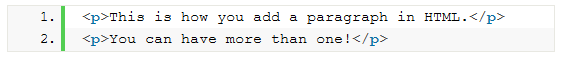
\includegraphics
	{../LaTeX/Images/html_element.PNG}
	\caption{Exemplu de element HTML}
	\label{fig:38}
\end{figure}

”p” vine de la paragraf. ”<p>” se mai numește ”opening tag” și definește punctul de intrare al elementului de tip paragraf și se poate observa că este închis între simbolurile ”<” și ”>”. ”</p>” reprezintă ”closing tag” și marchează punctul de ieșire al elementului, care, spre deosebire de punctul de intrare, mai are în componență simbolul ”/”. Textul sau conținutul paragrafului este definit între punctul de intrare și cel de ieșire. Un element HTML este format din toate cele 3 părți descrise mai sus.
\\ \\
%\label{css}
Acronimul CSS vine de la Cascading Style Sheets și reprezintă limbajul care permite determinarea aspectului unei pagini web, din punct de vedere vizual, schematic și estetic. Dacă HTML este planul unei case, CSS precizează stilul acesteia, Victorian sau Art Deco, Post-modern sau Gotic.
\\ \\
CSS schimbă aspectul paginii web interacționând cu elementele HTML. După cum am observat în (Fig. \ref{fig:38}), un paragraf este un asemenea element HTML. Dacă vrem ca textul paragrafului să fie de culoare roz și cu scris îngroșat, vom scrie codul CSS ilustrat în (Fig. \ref{fig:39}).

\begin{figure}[!htb]
	\centering
	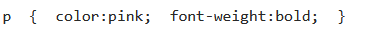
\includegraphics
	{../LaTeX/Images/css_paragraph.PNG}
	\caption{Exemplu de stilizare CSS}
	\label{fig:39}
\end{figure}

%maybe add \\ \\ here%
”p” se numește ”selector” și indică elementul HTML căruia îi vom schimba aspectul folosind reguli definite în CSS. ”color” și ”font-weight” sunt câteva dintre proprietățile de stilizare care se pot aplica selectorului de tip ”p”. Alte proprietăți ale acestuia sunt dimensiunea textului, adică ”font-size” sau ”text-transform” care poate transforma textul paragrafului în litere de tipar dacă se folosește împreună cu valoarea ”uppercase”.
\\ \\
Codul CSS poate fi adăugat unei pagini web în 3 moduri: intern, extern sau inline. În modul intern, codul CSS este scris în elementul HTML ”<style>”, ilustrat în (Fig. \ref{fig:311}).

\begin{figure}[!htb]
	\centering
	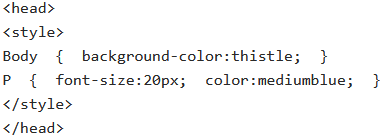
\includegraphics
	{../LaTeX/Images/css_internal.PNG}
	\caption{Modul intern de legare a codului CSS}
	\label{fig:311}
\end{figure}

Extern înseamnă scrierea codului într-un fișier separat salvat cu extensia ”.css”. Legătura dintre pagina web și regulile de stilizare din fișier se creează folosind elementul ”<link>”, după cum se poate observa în (Fig. \ref{fig:312}).

\begin{figure}[!htb]
	\centering
	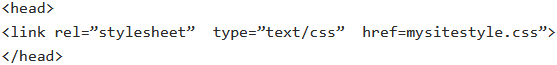
\includegraphics
	{../LaTeX/Images/css_external.PNG}
	\caption{Modul extern de legare a codului CSS}
	\label{fig:312}
\end{figure}

Codul ”inline” este codul CSS scris înăuntrul elementelor HTML, folosind proprietatea ”style”, reprezentat în (Fig. \ref{fig:313}).

\begin{figure}[!htb]
	\centering
	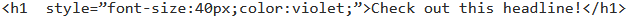
\includegraphics
	{../LaTeX/Images/css_inline.PNG}
	\caption{Modul inline de legare a codului CSS}
	\label{fig:313}
\end{figure}

Se preferă scrierea regulilor de stilizare într-un fișier separat deoarece astfel rezultă o separare între structura paginii web, elementele HTML și aspectul acesteia, regulile CSS. Codul este mai ușor de citit, mai ușor de întreținut și actualizat și permite o detectare mai ușoară a erorilor.
\\ \\
SCSS vine de la Sassy CSS și este un limbaj de preprocesare al cărui rezultat de compilare este cod CSS. În CSS este dificilă scrierea de reguli organizate și ușor de menținut deoarece lipsește suportul pentru cod imbricat (din engl. ”nested”), funcții și moștenire. Folosind SCSS se poate evita scrierea codului duplicat, prin construirea de bucăți de cod reutilizabile și se pot scrie secvențe de cod imbricate, care sunt structurate și ușor de citit (Fig. \ref{fig:314}).
\\ \\

\begin{figure}[!htb]
	\centering
	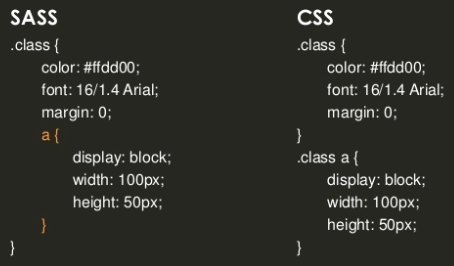
\includegraphics
	{../LaTeX/Images/scss_nesting.PNG}
	\caption{Secvență de cod ”nested”}
	\label{fig:314}
\end{figure}

Simbolul ”.” din ”.class” reprezintă o clasă de reguli de stilizare care se poate aplica unuia sau mai multor elemente HTML, spre deosebire de simbolul ”\#” care definește o regulă aplicabilă în mod unic unui singur element.
După cum se poate observa în (Fig. \ref{fig:314}), codul ”nested” evită dublarea selectorului ”.class” atunci când se face referire la elementul ”<a>”, de tip ancoră.
\\ \\
SCSS oferă suport pentru așa numitele ”directive de control”, care pot defini o regulă de stilizare dacă o anumită condiție este îndeplinită. Una dintre aceste directive este ”@if” care funcționează asemenea structurilor alternative din limbajele de programare precum C\#. Folosind ”@if”, se aplică unui element ”<div>” o margine albă de grosime de 1 pixel, dacă rezultatul condiției este egal cu 4, după cum este ilustrat în (Fig. \ref{fig:315}).

\begin{figure}[!htb]
	\centering
	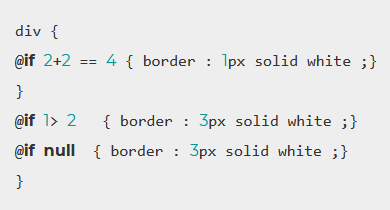
\includegraphics[width=0.4\textwidth]
	{../LaTeX/Images/scss_if-1.PNG}
	\caption{Directiva de control ”@if”}
	\label{fig:315}
\end{figure}

După evaluarea condiției din ”@if” și compilarea codului, rezultă regula de stilizare reprezentată în (Fig. \ref{fig:316}).

\begin{figure}[!htb]
	\centering
	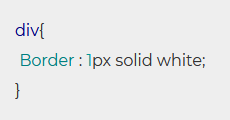
\includegraphics[width=0.2\textwidth]
	{../LaTeX/Images/scss_if-2.PNG}
	\caption{Directiva de control ”@if”}
	\label{fig:316}
\end{figure}
	
	\chapter{Framework-uri web}
	% !TeX root = ../FoodSpy.tex
% \section{Framework-uri web}

\section{Angular}
Numele ”Angular” vine de la caracterele ”<” și ”>” (în engleză, ”angled brackets”) care delimitează numele tuturor tag-urilor din HTML, de exemplu ”<a>” sau ”<div>”.
Angular este o platformă de dezvoltare, bazată pe limbajul TypeScript, care este un superset al limbajului JavaScript. Angular este un framework care face posibilă implementarea într-un mod trivial a cerințelor complexe ale aplicațiilor web, cum ar fi animații sau ”data binding”.
\\ \\
Platforma Angular oferă un mod de lucru bazat pe componente individuale care duce cu ușurință la construirea de aplicații web scalabile, dar și la posibilitatea reutilizării acestor componente în alte aplicații.
Angular vine integrat cu o multitudine de biblioteci care acoperă o gamă largă de cazuri de utilizare, printre care comunicarea cu un server și validarea formularelor HTML (Fig. \ref{fig:41}).

\begin{figure}[!htb]
	\centering
	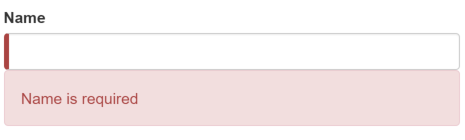
\includegraphics
	{../LaTeX/Images/angular_hero-form-2.PNG}
	\caption{Validarea câmpului ”Name” din formular}
	\label{fig:41}
\end{figure}

Mai mult, Angular este gândit să faciliteze actualizarea cât mai ușoară a aplicației, de aceea pune la dispoziție o suită de unelte care ajută la dezvoltarea, testarea și actualizarea codului printre care și ”Live Reload”, o funcționalitate prin care aplicația web este recompilată și deservită la orice modificare a codului-sursă.

\subsection{Components}
Asemenea blocurilor de LEGO, componentele Angular sunt puse laolaltă pentru a construi o aplicație web. O componentă (Fig. \ref{fig:42}) este formată dintr-o clasă TypeScript, adnotată cu decoratorul ”@Component”, un șablon HTML și opțiuni de stilizare.
\\ \\
În clasa TypeScript este scris codul care determină funcționalitatea componentei, șablonul HTML spune cum este structurată componenta, iar opțiunile de stilizare definesc aspectul acesteia. Această separare ajută la testarea mai ușoară a codului și lizibilitatea acestuia.

\begin{figure}[!htb]
	\centering
	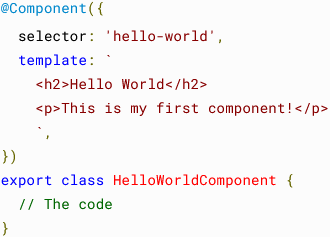
\includegraphics
	{../LaTeX/Images/angular_components.PNG}
	\caption{O componentă Angular}
	\label{fig:42}
\end{figure}

Componenta se folosește printr-un apel după numele descris sub proprietatea ”selector”, în cazul acesta ”<hello-world></hello-world>”.

\subsection{Templates}
”Template” sau ”șablonul” descrie felul în care este structurată componenta folosind limbaj HTML. Limbajul HTML poate fi scris ”inline”, cum se vede în (Fig. \ref{fig:42}) sub proprietatea ”template” sau poate fi scris într-un fișier separat cu extensia ”.html”.
Angular extinde capabilitățile limbajului HTML oferind așa numitele ”directives”, care sunt clase ce pot modifica în mod dinamic structura aplicației.
\\ \\
De exemplu, ”*ngIf” poate fi folosit pe un ”<div>” (dar și alte tag-uri HTML) pentru a-l afișa sau nu în funcție de valoarea unei variabile de tip ”boolean”, astfel:

\begin{verbatim}
	<div *ngIf=”showDiv”>
	<p> Dacă ”showDiv” este ”true” atunci ”<div>” este vizibil în pagină </p>
	</div>
	
	<div *ngIf=”!showDiv”>
	<p> Dacă ”showDiv” este ”false” atunci ”<div>” nu este vizibil în pagină </p>
	</div>
\end{verbatim}

De reținut este faptul că ”showDiv” este o variabilă ce a fost definită în clasa TypeScript a componentei.

\subsection{Dependency Injection}
Prin ”dependency injection” a se înțelege un design pattern prin care este posibilă scrierea de cod-sursă mai flexibil și mai ușor de testat. În Angular, prin ”dependency injection”, într-o clasă se pot declara dependințe către alte clase, fără să fie necesară instanțierea explicită a lor - instanțierea se efectuează în mod automat.
O clasă către care este definită o dependință din altă clasă trebuie să fie adnotată cu decoratorul ”@Injectable”, astfel:

\begin{figure}[!htb]
	\centering
	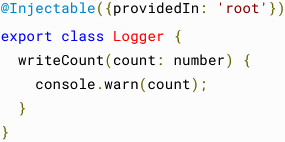
\includegraphics
	{../LaTeX/Images/angular_injectable.PNG}
	\caption{”Logger” este o clasă ce poate fi ”injectată”}
	\label{fig:44}
\end{figure}

Funcția ”writeCount()” din clasa ”Logger” este folosită mai departe în interiorul clasei ”HelloWorldDependencyInjectionComponent”, după cum se vede în (Fig. \ref{fig:45}).

\begin{figure}[!htb]
	\centering
	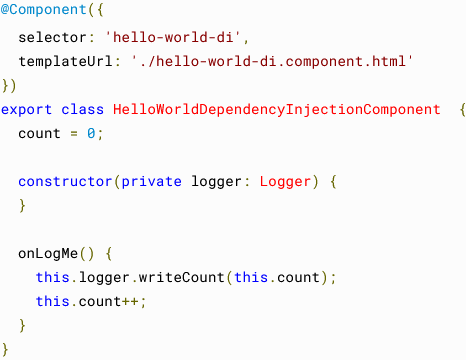
\includegraphics
	{../LaTeX/Images/angular_dependency-injection.PNG}
	\caption{”HelloWorldDependencyInjectionComponent” cu membrul ”private logger”}
	\label{fig:45}
\end{figure}

A se observa constructorul clasei ”HelloWorldDependencyInjectionComponent”, unde s-a definit o dependință către clasa ”Logger” prin membrul ”private logger”.

\section{ASP.NET Core}
ASP.NET Core este un framework web, care rulează pe platforma .NET și .NET Core. Bazat pe limbajul de programare C\#, ASP.NET Core suportă construirea serviciilor REST (așa numitele API-uri web).
Un ”request” sau o ”cerere” venită către un asemenea serviciu REST este tratată de către un controller. În ASP.NET Core, un controller este o clasă ce derivă din clasa de bază ”ControllerBase”.

\begin{figure}[!htb]
	\centering
	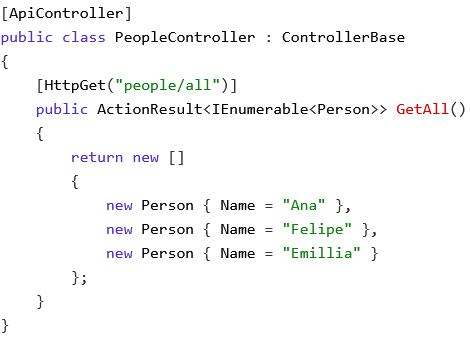
\includegraphics[width=0.8\textwidth]
	{../LaTeX/Images/asp_controller-1.PNG}
	\caption{”PeopleController” este un exemplu de controller}
	\label{fig:46}
\end{figure}

Deoarece ”PeopleController” este adnotat cu atributul ”[HttpGet("people/all")]”, acesta este capabil să răspundă cererilor metodei ”GET” efectuate la URL-ul ”/people/all”.
\\ \\
”people/all” se mai numește ”endpoint” și intrinsec este configurat să răspundă într-un mod serializabil, sub forma unui JSON, după cum se poate observa în (Fig. \ref{fig:47}).

\begin{figure}[!htb]
	\centering
	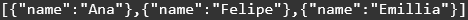
\includegraphics
	{../LaTeX/Images/asp_response.PNG}
	\caption{Exemplu de răspuns dat de un controller}
	\label{fig:47}
\end{figure}

După cum se poate observa și în exemplele de mai sus, ASP.NET Core permite definirea ”inline” a endpoint-urilor și metodelor REST prin adnotări, folosind atribute.
Un exemplu de controller capabil să răspundă la metodele ”GET” și ”POST” este ilustrat în (Fig. \ref{fig:48}).

\begin{figure}[!htb]
	\centering
	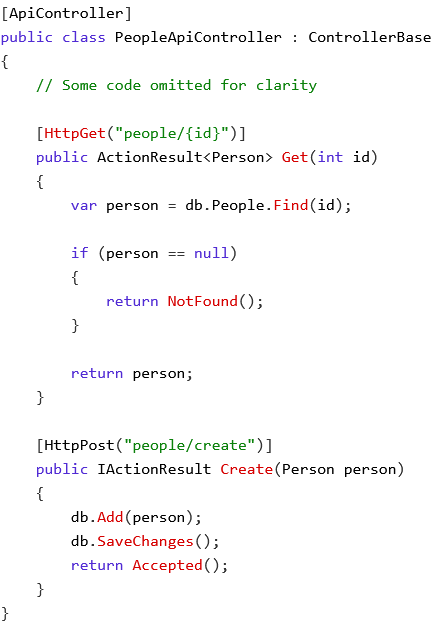
\includegraphics[width=0.8\textwidth]
	{../LaTeX/Images/asp_controller-2.PNG}
	\caption{Exemplu controller}
	\label{fig:48}
\end{figure}

În practică deci, un web API construit folosind ASP.NET Core nu este altceva decât o colecție de unul sau mai multe controller-e care sunt capabile să răspundă cererilor venite din partea interfeței-utilizator (și nu numai).
	
	\chapter{Tehnologii}
	% !TeX root = ../FoodSpy.tex
% \section{Tehnologii}

\section{MikroORM și ORM}
ORM sau Object-Relational Mapping este o tehnică de a interoga și manipula datele dintr-o bază de date folosind o paradigmă orientată pe obiect. MikroORM este o bibliotecă TypeScript care implementează această tehnică.
MikroORM încapsulează codul necesar manevrării datelor și astfel nu mai este nevoie de scrierea explicită a interogărilor.
\\ \\
Mai mult, biblioteca permite interacțiunea directă cu obiectele din baza de date folosind același limbaj în care este scris codul-sursă al aplicației - în cazul nostru, TypeScript.
\\ \\
MikroORM prezintă o serie de avantaje printre care faptul că utilizarea procedurilor stocate sau a tranzacțiilor se face la fel de simplu precum un apel de funcție, dar și faptul că modelul de date este definit o singură dată, ceea ce îl face ușor de actualizat și menținut. Un exemplu de model de date este ”User”. ”User” modelează utilizatorul aplicației, prin câmpuri precum ”email”, și este reprezentat în (Fig. \ref{fig:51}).

\begin{figure}[!htb]
	\centering
	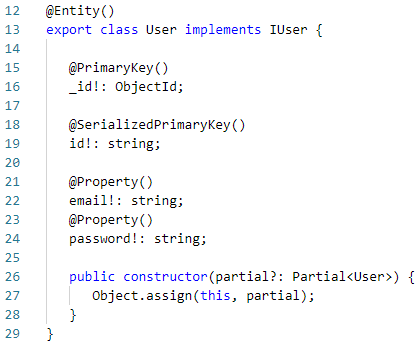
\includegraphics
	{../LaTeX/Images/mikroorm_user.PNG}
	\caption{Model de date MikroORM}
	\label{fig:51}
\end{figure}


\section{MongoDB și MongoDB Atlas}
MongoDB este un sistem de gestiune a bazelor de date orientat pe document. Deoarece un document este asemenea unui obiect JSON, câmpurile conținute în acesta pot să difere de la document la document și de asemenea, structura acestuia se poate modifica de-a lungul timpului. MongoDB permite o asociere directă între documentul din baza de date și obiectul din codul-sursă al aplicației, oferind programatorului posibilitatea de a manipula datele cu ușurință.

\begin{figure}[!htb]
	\centering
	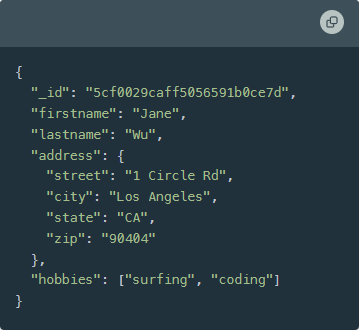
\includegraphics
	{../LaTeX/Images/mongodb_document.PNG}
	\caption{Document MongoDB}
	\label{fig:52}
\end{figure}

%maybe add \\ \\ here
La rădăcini, MongoDB este un sistem de gestiune scalabil și pretabil pentru a rula pe sisteme distribuite - aici intervine MongoDB Atlas care este serviciul MongoDB găzduit în cloud. Atlas pune la dispoziție toate funcționalitățile serviciului MongoDB, dar în același timp automatizează partea de administrare a bazei de date, de la configurarea acesteia până la efectuarea operației de ”backup”.
\\ \\
În oferta de găzduire în cloud există și un nivel gratis, așa numitul ”M0 Sandbox”, care poate fi folosit pentru acomodare cu serviciul MongoDB, pentru prototipare și pentru primele implementări ale bazei de date.


\section{Node.js}
Node.js este un mediu de rulare JavaScript construit pe engine-ul V8 din Chrome. Este folosit pentru a rula aplicații web în afara browser-ului clientului. Deoarece folosește un mediu de rulare asincron, bazat pe evenimente, Node.js este gândit pentru scalabilitatea aplicațiilor de rețea, fiind capabil să administreze un număr mare de conexiuni în mod concurent.
\\ \\
Un modul Node.js este asemenea unei librării JavaScript care poate fi inclus înăuntrul unei aplicații pentru a facilita anumite funcționalități. De exemplu, în (Fig. \ref{fig:53}) este ilustrată utilizarea modului HTTP care face posibil crearea unui server web, care ascultă pe portul 2000.

\begin{figure}[!htb]
	\centering
	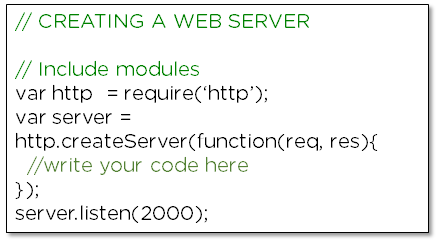
\includegraphics[width=0.6\textwidth]
	{../LaTeX/Images/nodejs_http.PNG}
	\caption{Modulul HTTP din Node.js}
	\label{fig:53}
\end{figure}

Față de mediul de rulare convențional, bazat pe thread-uri, Node.js are avantajul că funcțiile nu execută operații de input / output, deci procesul de rulare al aplicației nu este blocat niciodată. Mai mult, librăria Express din Node.js poate fi utilizată în diferite scenarii, de la aplicații de chat în timp real până la API-uri REST.


\section{Express}
Node.js nu oferă suport pentru diferitele verbe HTTP, precum GET, POST sau DELETE. De asemenea, nu poate servi fișiere statice și nici nu poate trata cererile care pot veni la diferite URL-uri, așa numitele ”rute” sau ”endpoint”-uri. Pentru aceste cazuri, este necesară implementarea manuală sau folosirea unui framework web, în speță, Express.
\\ \\
Express adresează neajunsurile Node.js enumerate mai sus prin pachete ”middleware” și mai mult decât atât, aceste pachete pot fi folosite pentru lucrul cu sesiuni sau cookie-uri, extragerea parametrilor din URL sau a datelor transmise prin corpul cererilor POST.

\begin{figure}[!htb]
	\centering
	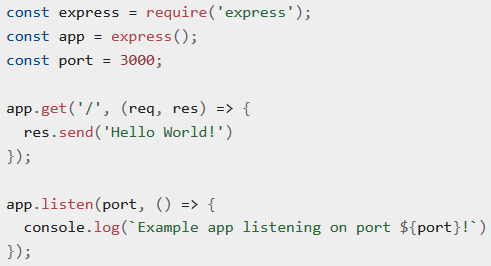
\includegraphics
	{../LaTeX/Images/express_hello.PNG}
	\caption{”Hello World” în Express}
	\label{fig:54}
\end{figure}

%maybe add \\ \\ here
Inițial, se importă modulul Express prin ”require(‘express’)”. Aplicația Express se instanțiază prin ”const app = express()”. Cu ajutorul ”app” definim ”endpoint”-urile tratate de API. În cazul prezentat în (Fig. \ref{fig:54}), ”app.get()” definește o funcție care va fi apelată atunci când se face un request GET la URL-ul rădăcină, adică ”/”. Răspunsul se trimite înapoi folosind ”send()” și va întoarce string-ul ”Hello World”. Cu ”app.listen()” se pornește server-ul care ascultă pe portul 3000 și care poate fi accesat la adresa ”localhost:3000”.


\section{NPM și publicarea pachetului ”FoodSpy-shared”}
NPM este manager-ul de pachete pentru Node.js. A fost creat în 2009 ca un proiect care să ajute dezvoltatorii JavaScript să partajeze cu ușurință secvențe de cod sub formă de module [REF](referință către Node.js) ambalate ca pachete. Registrul NPM este o colecție publică de astfel de pachete care sunt folosite de către comunitatea JavaScript pentru dezvoltarea aplicațiilor web sau aplicațiilor mobile. NPM pune la dispoziție un client care poate fi folosit în linie de comandă și oferă dezvoltatorilor capabilitatea de a instala, folosi și de a publica propriile pachete.
\\ \\
”FoodSpy-shared” este un pachet propriu, disponibil în registrul public NPM. Acesta conține o colecție de constante, interfețe și enum-uri folosite în aplicația Angular, dar și în API-ul care administrează datele despre utilizatori. Una dintre aceste interfețe este ”IUser”, ilustrată în (Fig. \ref{fig:55}). ”IUser” definește contractul care trebuie îndeplinit atât pe partea de front-end cât și pe partea de back-end, când vine vorba de manipularea datelor despre un utilizator. Adăugarea pachetului ”FoodSpy-shared” și implementarea interfeței ”IUser” în API este ilustrată în (Fig. \ref{fig:56}).

\begin{figure}[!htb]
	\centering
	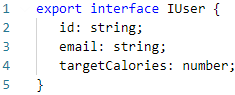
\includegraphics
	{../LaTeX/Images/npm_iuser.PNG}
	\caption{Interfața ”IUser”}
	\label{fig:55}
\end{figure}

\begin{figure}[!htb]
	\centering
	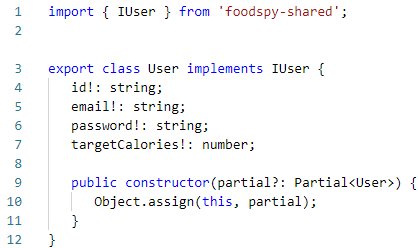
\includegraphics
	{../LaTeX/Images/npm_user.PNG}
	\caption{Implementarea interfeței ”IUser” în API}
	\label{fig:56}
\end{figure}


\section{Heroku}
Heroku este o platformă care pune la dispoziție posibilitatea de a construi, implementa și rula aplicații găzduite în cloud. Spre deosebire de Amazon Web Services sau Windows Azure, care oferă doar infrastructura în cloud necesară pentru a găzdui aplicația, Heroku oferă un serviciu de management asupra infrastructurii, care abstractizează toate detaliile legate de configurare și implementare. Astfel, Heroku permite dezvoltatorilor să concentreze toate resursele spre implementarea aplicației.
Heroku suportă o colecție de limbaje de programare și framework-uri, printre care JavaScript și Node.js.
\\ \\
Platforma pune la dispoziție toate uneltele necesare implementării unei aplicații, inclusiv administrarea mediului de rulare a aplicației și administrarea laturii DevOps. Din acest motiv, Heroku este un loc potrivit pentru a învăța despre microservicii și metodologii de implementare, precum livrarea continuă (”continuous delivery”). Mai mult decât atât, oferă un abonament destinat exclusiv studenților care permite utilizarea platformei pentru o perioadă de doi ani, suficient timp pentru a exersa orice limbaj de programare și orice șablon arhitectural.


\section{Utilitare (Postman, Git și GitHub)}
Postman este un utilitar interactiv prin care se pot examina endpoint-urile unui API. Postman poate fi folosit pe tot parcursul dezvoltării unei aplicații deoarece dispune de o interfață grafică care permite construirea și trimiterea de request-uri HTTP. De asemenea, se poate folosi pentru citirea și validarea răspunsurilor oferite de către API. Un exemplu de request trimis direct din Postman către ”FoodSpyAPI”, care interoghează baza de date pentru alimente care au în componența numelui termenul ”magiun” este reprezentat în (Fig. \ref{fig:57}).

\begin{figure}[!htb]
	\centering
	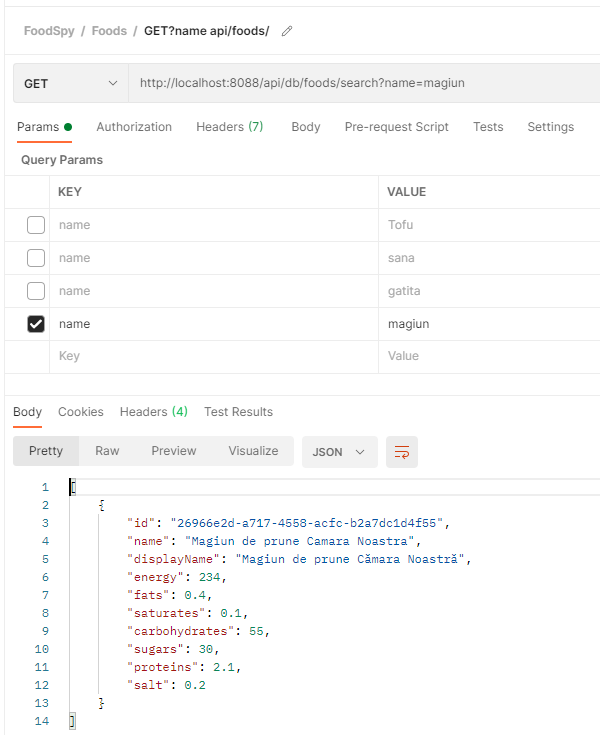
\includegraphics[width=0.8\textwidth]
	{../LaTeX/Images/postman_magiun.PNG}
	\caption{Request ”GET” trimis din Postman}
	\label{fig:57}
\end{figure}

%maybe add \\ \\ here
Git este un sistem de versionare distribuit care poate urmări schimbări în fișiere. Git este folosit de programatori pentru a colabora la scrierea codului-sursă în procesul de dezvoltare software. A fost creat în anul 2005 și a fost gândit pentru a fi eficient, pentru a păstra integritatea datelor și pentru a oferi suport pentru numeroase medii de dezvoltare.
\\ \\
Git urmărește schimbările în fișier pe toată durata dezvoltării software, ceea ce înseamnă că în orice moment, codul-sursă poate fi revizuit sau poate fi adus la o versiune precedentă.
\\ \\
Git se instalează și rulează pe sistemul local și nu are nevoie de conexiune la internet pentru a funcționa. Față de alte sisteme de versionare, Git este ușor de folosit și gratis și a fost gândit să lucreze în principal cu fișiere text, adică exact tipul de fișiere folosit pentru a salva cod-sursă. Întregul cod-sursă este menținut sub evidența sistemului de versionare într-un director care poartă numele de ”repository”. Avantajul major al Git este așa numitul ”branching model”. Prin procesul de ”branching” se pot crea ”ramuri”, care sunt copii independente ale repository-ului. Asta se traduce prin ușurința de a testa și implementa noi funcționalități în aplicație, fără a afecta munca celorlalți participanți la dezvoltarea aplicației.
\\ \\
GitHub este un serviciu de găzduire a unui repository. Este bazat exclusiv pe infrastructură cloud și este o bază de date care reține o colecție de repository-uri. GitHub este practic o versiune online a unui repository local și astfel oferă posibilitatea de a partaja un repository sau de a adăuga alți programatori care pot contribui în mod independent la dezvoltarea aplicației. Cu alte cuvinte, GitHub extinde funcționalitățile oferite de Git printr-o interfață intuitivă și unelte de management asupra unui repository. Un instantaneu al repository-ului care conține codul-sursă al aplicației ”FoodSpy” este reprezentat în (Fig. \ref{fig:58}). Se poate observa că branch-ul ”calculate-calories” a suferit 9 modificări de la momentul în care a fost clonat din branch-ul principal, adică ”master”.

\begin{figure}[!htb]
	\centering
	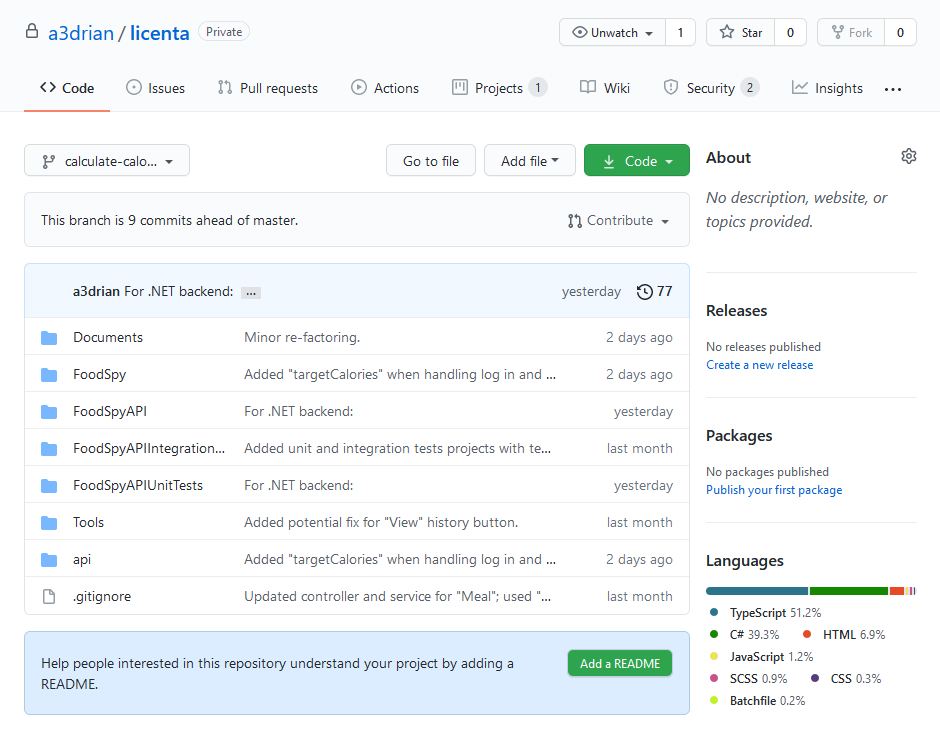
\includegraphics[width=0.9\textwidth]
	{../LaTeX/Images/github_repo.PNG}
	\caption{Repository-ul ”FoodSpy”}
	\label{fig:58}
\end{figure}
	
	\chapter{Descrierea aplicației}
	% !TeX root = ../FoodSpy.tex
% \section{Descrierea aplicației}

\begin{figure}[!htb]
	\centering
	
\includegraphics[width=0.8\textwidth]
	{../LaTeX/Images/implementare_arhitectura.PNG}
	\caption{Arhitectura aplicației FoodSpy}
	\label{fig:61}
\end{figure}

Arhitectura aplicației FoodSpy presupune o implementare realizată pe mai multe nivele de infrastructură, nivele ce sunt detaliate în rândurile următoare.
\\ \\
Proiectul ”FoodSpy” reprezintă nivelul clientului sau nivelul de prezentare, adică interfața grafică prin care utilizatorul interacționează cu aplicația.
\\ \\
”FoodSpyUserAPI” este interfața de programare care efectuează comunicarea cu server-ul care se ocupă de administrarea utilizatorilor și a datelor acestora.
\\ \\
Proiectul care se ocupă de persistența datelor reținute în jurnalul fiecărui utilizator este ”FoodSpyAPI”. Acesta este responsabil pentru stocarea informațiilor legate de mâncărurile pe care utilizatorii le pot folosi pentru a-și compune mesele și pentru a înregistra aportul caloric în jurnal.
\\ \\
Nivelul de testare este acoperit de proiectele ”FoodSpyAPIIntegrationTests” și ”FoodSpyAPIUnitTests”.
\\ \\
”foodspy-shared” este proiectul care reprezintă nivelul auxiliar, un nivel care face posibilă partajarea dependințelor aplicației. Acesta conține o colecție de enumerări și interfețe care sunt folosite atât la nivelul clientului cât și la nivelul interfețelor de programare (API-urilor).

\section{Clientul}
Nivelul clientului este împărțit pe mai multe componente Angular.
\\ \\
”Auth” constituie componenta care administrează pagina de autentificare în aplicație. La baza acestei componente este un formular HTML. Pentru un utilizator care urmează să își creeze un cont, formularul are 3 câmpuri: e-mail-ul, parola și aportul zilnic de calorii pe care acesta dorește să-l atingă în fiecare zi. Pentru e-mail se folosește o validare bazată pe o expresie regulată care impune în componența sa existența unui domeniu (”.com”, ”.ro”, etc.). Parola trebuie să aibă un număr minim de caractere, număr definit de o constantă, iar aportul este exprimat ca un număr întreg cuprins într-un anumit interval.
\\ \\
Pentru cazul în care utilizatorul are deja cont și efectuează operația de autentificare în aplicație, formularul nu mai afișează câmpul numărului de calorii.
Se observă astfel faptul că același formular este folosit pentru procesul de înregistrare, dar și pentru procesul de autentificare. Această implementare este posibilă folosind directiva ”*ngIf”.

\begin{figure}[!htb]
	\centering
	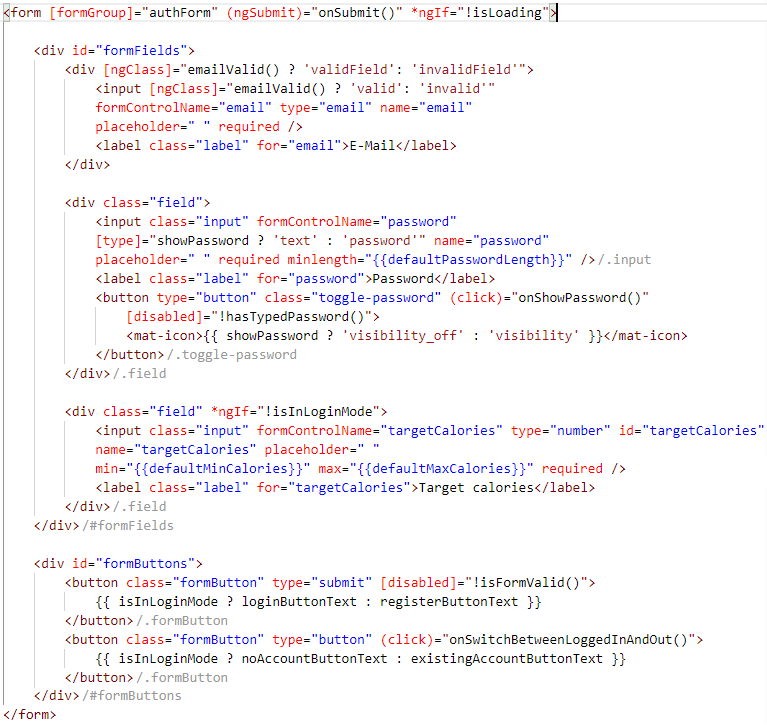
\includegraphics[width=0.95\textwidth]
	{../LaTeX/Images/implementare_form.PNG}
	\caption{Formularul de înregistrare și autentificare în aplicație}
	\label{fig:62}
\end{figure}

”Auth” utilizează serviciul de autentificare ”AuthService”. Acesta validează datele introduse în formular și trimite un request ”POST” către interfața de programare care se ocupă de administrarea utilizatorilor. Request-ul ”POST” este împachetat într-o interfață ”IAuthResponseData” compusă din proprietățile ”email”, ”password” și ”targetCalories”. Interfața este partajată cu ”FoodSpyUserAPI” pentru a facilita despachetarea cu ușurință a informațiilor conținute în request-ul ”POST”.

\begin{figure}[!htb]
	\centering
	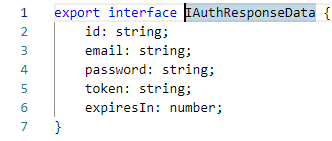
\includegraphics
	{../LaTeX/Images/implementare_iauthresponsedata.PNG}
	\caption{Interfața ”IAuthResponseData”}
	\label{fig:63}
\end{figure}

După înregistrare sau autentificare, utilizatorul este redirecționat către componenta ”Intakes”. ”Intakes” reprezintă tabloul de bord al aplicației și afișează numărul de calorii pe care acesta și le-a setat ca obiectiv de atins la momentul înregistrării.
De asemenea, oferă posibilitatea de a urmări istoricul utilizării aplicației, pe zile, ordonate de le cea mai îndepărtată zi, la cea mai apropiată. Acest istoric reprezintă de fapt jurnalul aportului de calorii al utilizatorului.

\begin{figure}[!htb]
	\centering
	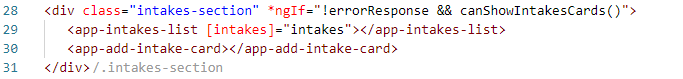
\includegraphics[width=0.9\textwidth]
	{../LaTeX/Images/implementare_intakes.PNG}
	\caption{Componenta ”Intakes”}
	\label{fig:64}
\end{figure}

Obiectul ”intakes” de la linia 29 din (Fig. \ref{fig:64}) este populat cu rezultatul unui request ”POST” către ”FoodSpyAPI” care întoarce o listă de intrări din jurnalul unui anume utilizator, identificat prin adresa acestuia de e-mail. 
Nu se face un request ”GET” deoarece acest endpoint din (Fig. \ref{fig:65}) permite sortarea intrărilor din jurnal, din punct de vedere cronologic, dacă se populează o proprietate numită ”sortOrder” cu valoarea 0 pentru ascendent sau cu valoarea 1 pentru descendent.

\begin{figure}[!htb]
	\centering
	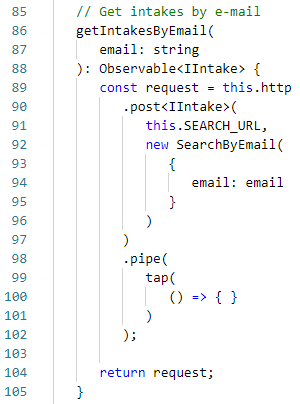
\includegraphics[width=0.6\textwidth]
	{../LaTeX/Images/implementare_getintakesbyemail.PNG}
	\caption{Request ”POST” către ”/api/db/intakes/search/”}
	\label{fig:65}
\end{figure}

În tabloul de bord, fiecare dintre aceste zile care face parte din istoric sunt conținute într-o componentă numită ”IntakeCard”. În ”IntakeCard”, istoricul nu este detaliat, afișează doar procentul de completare al aportului de calorii, și cantitatea totală de grăsimi, carbohidrați și zaharuri pe care utilizatorul le-a consumat în ziua respectivă.
\\ \\
Detaliile precum mâncărurile care fac parte din componența unei mese și cantitatea fiecăruia dintre mâncăruri consumate de utilizator sunt afișate în componenta ”IntakeHistory”, la care se ajunge prin intermediul unui hyperlink. Hyperlink-ul este atașat unei element ”<h2>” prin evenimentul ”(click)”, după cum se poate observa în (Fig. \ref{fig:66}). Elementul ”<h2>” exprimă numărul de mese consumate de utilizator într-o anumită zi.

\begin{figure}[!htb]
	\centering
	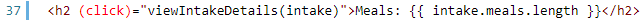
\includegraphics[width=0.95\textwidth]
	{../LaTeX/Images/implementare_hyperlink.PNG}
	\caption{Hyperlink atașat pe evenimentul ”(click)”}
	\label{fig:66}
\end{figure}

”Intakes” face legătură către ”AddMeal” prin componenta ”AddIntakeCard”. Cu ajutorul ”AddMeal”, un utilizator poate căuta mâncărurile pe care să la adauge la o masă, iar masa o poate adăuga la jurnalul din ziua respectivă.
\\ \\
”AddMeal” este cea mai complicată dintre componente, deoarece ea implementează funcționalitatea pentru căutarea mâncărurilor în baza de date și construcția unui obiect de tip ”IIntake”, care reprezintă o zi din jurnal.
\\ \\
Când utilizatorul accesează componenta ”AddMeal”, se inițializează obiectul de tip ”IIntake” cu valori default. De exemplu, o proprietate a acestui obiect este ”createdAt”, care va reține momentul la care s-a adăugat în jurnal prima masă. Se mai inițializează proprietatea ”email” cu e-mail-ul utilizatorului și ”targetCalories” cu obiectivul setat de utilizator.

\begin{figure}[!htb]
	\centering
	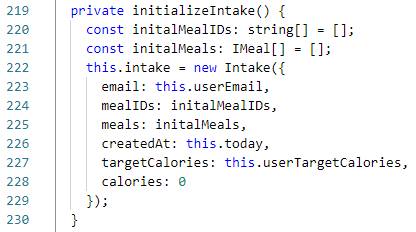
\includegraphics[width=0.8\textwidth]
	{../LaTeX/Images/implementare_initializeintake.PNG}
	\caption{Inițializarea componentei ”Intakes”}
	\label{fig:67}
\end{figure}

Căutarea mâncărurilor din baza de date se face folosind un ”<input>” de tip ”text” atașat la o funcție care preia termenul de căutare introdus de către utilizator și face un request ”GET” către ”FoodsService”. Termenul de căutare populează parametrul din URL numit ”name” și asta va determina endpoint-ul definit în ”FoodSpyAPI” să returneze o listă de mâncăruri filtrate după nume. Un exemplu de request ”GET” după criteriul numelui este ”/api/db/foods/search?name=ciocolata”.

\begin{figure}[!htb]
	\centering
	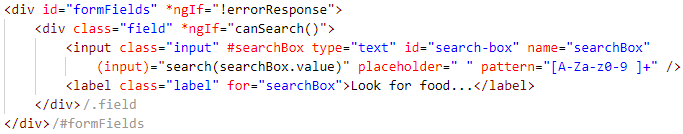
\includegraphics[width=0.9\textwidth]
	{../LaTeX/Images/implementare_search.PNG}
	\caption{Bara de căutare a mâncărurilor după nume}
	\label{fig:68}
\end{figure}

Odată găsită mâncarea în baza de date, utilizatorul poate deschide o căsuță de dialog, care reprezintă componenta ”EditFoodDialogue”. Aici, utilizatorul poate vedea mai multe detalii despre mâncarea selectată în urma căutării, printre care cantitatea de săruri sau proteine și de asemenea poate introduce cantitatea de mâncare, exprimată în grame.
\\ \\
Pentru cantitate este construită o validare care impune valoarea acesteia să nu poată depăși 1000 de grame. Validarea este ilustrată în (Fig. \ref{fig:69}). Aceasta poartă numele de ”foodQuantityValidator” și este implementată folosind clasa abstractă ”AbstractControl”. ”AbstractControl” permite accesul la valoarea introdusă de utilizator în formular și astfel se pot impune restricții asupra acesteia.

\begin{figure}[!htb]
	\centering
	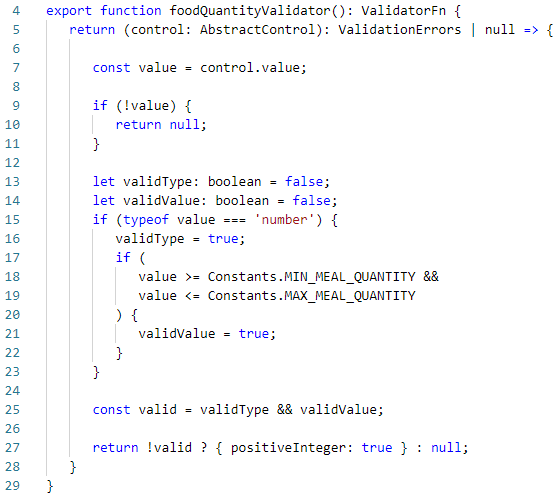
\includegraphics[width=0.9\textwidth]
	{../LaTeX/Images/implementare_foodqtyvalidator.PNG}
	\caption{Validarea pentru cantitatea de mâncare}
	\label{fig:69}
\end{figure}

După adăugarea unei mâncăruri, utilizatorul poate selecta tipul de masă pe care acesta a consumat-o. Tipurile de masă sunt ”Breakfast”, ”Lunch”, ”Dinner” sau ”Snack”. La momentul alegerii unuia dintre tipuri, formularul este valid și utilizatorului i se permite să înregistreze masa în jurnal.
\\ \\
Când se înregistrează o masă, există două scenarii.
\\ \\
Primul scenariu este acela în care utilizatorul nu are nicio intrare în jurnalul zilei respective, iar al doilea scenariu reprezintă modificarea unui jurnal deja existent.
În primul scenariu, implementarea este simplă deoarece este suficient să adăugăm masa în colecția ”Meals” din baza de date și apoi să introducem ID-ul acestei mese în proprietatea ”mealIDs” a obiectului de tip ”IIntake”. Ultimul pas este să trimitem un request ”POST” către ”FoodSpyAPI” pentru a înregistra jurnalul în colecția ”Intakes” din baza de date.
\\ \\
Al doilea scenariu este mai complicat deoarece în primul rând trebuie să determinăm dacă această masă nou adăugată face parte dintr-un tip de masă care există deja în în obiectul ”IIntake”.
Dacă nu face parte, se persistă o masă nouă și se aduce referința în proprietatea ”mealIDs” prin ID, iar în final se execută un request ”PUT” pentru a modifica un ”Intake” deja existent. Dacă face parte, atunci trebuie identificată colecția de mese care are același tip cu tipul mesei pe care utilizatorul dorește să o adauge. După identificarea acesteia, se concatenează colecția existentă cu masa ce urmează să fie adăugată, se aduce referința (ID-ul) în obiectul ”IIntake” și din nou se modifică jurnalul (obiectul de tip ”IIntake”) prin același request ”PUT”.
\\ \\
După executarea oricăruia dintre cele 2 scenarii descrise mai sus, se reîncarcă pagina pentru a reflecta modificarea din obiectul ”IIntake”.

\begin{figure}[!htb]
	\centering
	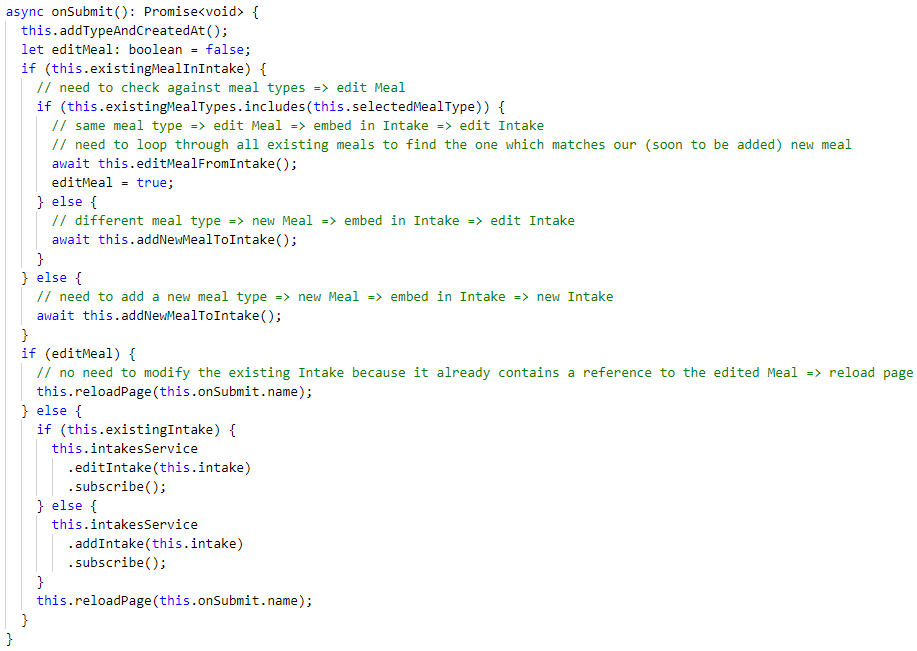
\includegraphics[width=0.95\textwidth]
	{../LaTeX/Images/implementare_addmeal.PNG}
	\caption{Adăugarea unei intrări în jurnalul zilnic}
	\label{fig:610}
\end{figure}

Prezent deasupra tuturor celorlalte componente, ”Header” (Fig. \ref{fig:611}) reprezintă antetul aplicației. Acesta afișează e-mail-ul utilizatorului autentificat, logo-ul aplicației și un buton pe care utilizatorul îl poate folosi pentru deconectare și redirecționare la componenta ”Auth”.

\begin{figure}[!htb]
	\centering
	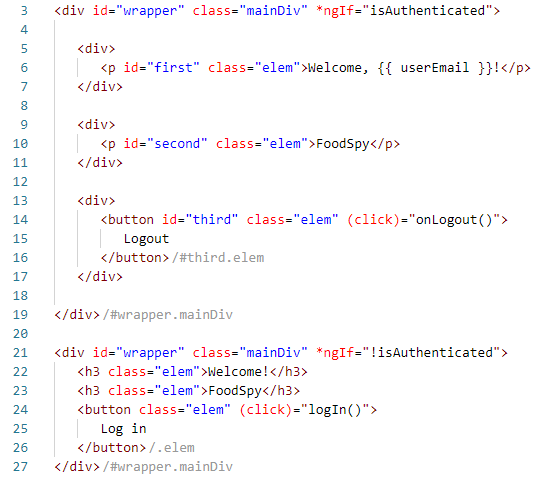
\includegraphics[width=0.8\textwidth]
	{../LaTeX/Images/implementare_header.PNG}
	\caption{Componenta ”Header”}
	\label{fig:611}
\end{figure}


\section{API pentru administrarea utilizatorilor}
Interfața de programare pentru administrarea utilizatorilor pune la dispoziție două endpoint-uri, un endpoint pentru operația de înregistrare a unui nou utilizator și unul pentru procesul de autentificare în aplicație.
\\ \\
La baza API-ului stă MikroORM, biblioteca TypeScript care implementează tehnica de a interoga și manipula datele dintr-o bază de date folosind o paradigmă orientată pe obiect. Cu ajutorul MikroORM, se definește o entitate care modelează profilul unui utilizator, dar și un manager peste această entitate care permite înregistrarea sau autentificarea acestuia în aplicație.
\\ \\
Pentru înregistrarea unui utilizator este nevoie să definim un endpoint pentru verbul ”POST” cu ajutorul unei rute. Din (Fig. \ref{fig:612}), se poate observa că ruta folosită pentru procesul de înregistrare este ruta rădăcină, adică ”/api/auth/register”.

\begin{figure}[!htb]
	\centering
	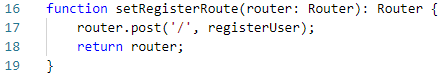
\includegraphics
	{../LaTeX/Images/userapi_rutaregister.PNG}
	\caption{Ruta pentru înregistrare}
	\label{fig:612}
\end{figure}

”registerUser” este funcția care face un apel către ”getUserByEmail” din ”UserService”. Funcția respectivă întoarce imediat o eroare dacă din corpul request-ului ”POST” lipsește e-mail-ul utilizatorului. Altfel, folosind manager-ul peste entități oferit de MikroORM, se caută utilizatorul identificat de e-mail-ul introdus în formularul din componenta ”Auth” din client. Dacă se găsește utilizatorul, detaliile despre acesta se returnează într-un obiect ”User”, iar dacă nu există, funcția întoarce ”null”.
\\ \\
În (Fig. \ref{fig:613}) este ilustrată funcția ”getUserByEmail”.

\begin{figure}[!htb]
	\centering
	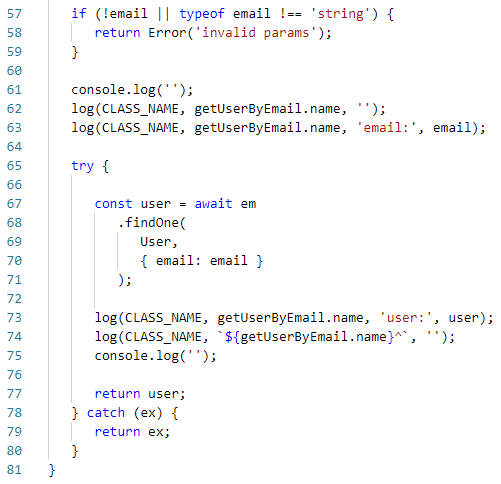
\includegraphics[width=0.9\textwidth]
	{../LaTeX/Images/userapi_getuserbyemail.PNG}
	\caption{Funcția ”getUserByEmail”}
	\label{fig:613}
\end{figure}

La momentul înregistrării, este important ca ”getUserByEmail” să returneze ”null”. Dacă returnează ”null”, înseamnă că utilizatorul nu există în baza de date și se poate înregistra cu succes folosind e-mail-ul, parola și obiectul caloric propus. Parola este criptată folosind biblioteca ”bcrypt” pentru a nu fi persistată în baza de date în format ”plain text”.
\\ \\
Dacă ”getUserByEmail” nu returnează ”null”, înseamnă că utilizatorului trebuie să îi fie afișat un mesaj de eroare care să-l atenționeze că există deja un cont creat cu același e-mail.

\begin{figure}[!htb]
	\centering
	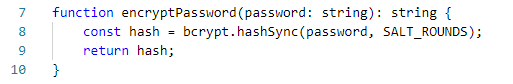
\includegraphics
	{../LaTeX/Images/userapi_bcrypt.PNG}
	\caption{Criptarea parolei folosind ”bcrypt”}
	\label{fig:614}
\end{figure}

Pentru autentificarea unui utilizator este nevoie să definim un endpoint pentru verbul ”POST” cu ajutorul unei rute. Din (Fig. \ref{fig:615}), se poate observa că ruta folosită pentru procesul de autentificare este ruta rădăcină, adică ”/api/auth/login”.

\begin{figure}[!htb]
	\centering
	\includegraphics
	{../LaTeX/Images/userapi_rutalogin.PNG}
	\caption{Ruta pentru autentificare}
	\label{fig:615}
\end{figure}

Asemenea funcției ”registerUser”, funcția ”loginUser” face un apel către ”getUserByEmail” din ”UserService”.
\\ \\
La momentul autentificării, această funcție trebuie să returneze un obiect ”User”, care conține datele despre utilizator. În caz contrar, există scenariul în care utilizatorul nu există și trebuie mai întâi să se înregistreze sau există scenariul în care utilizatorul se află în baza de date. În acest caz, parola introdusă în formular este comparată cu parola persistată, iar dacă nu există o potrivire, un mesaj de eroare este afișat în client.

\begin{figure}[!htb]
	\centering
	\includegraphics[width=0.9\textwidth]
	{../LaTeX/Images/userapi_loginuser.PNG}
	\caption{Corpul funcției ”loginUser”}
	\label{fig:616}
\end{figure}

La momentul pornirii server-ului care administrează datele despre utilizator, se caută un fișier numit ”.env” care conține string-ul de conectare la baza de date MongoDB precum și portul la care ascultă pentru cererile venite din partea clientului. ”.env” este interpretat de către API, care identifică string-ul de conectare și deschide portul de comunicare pentru client.
\\ \\
Fișierul ”.env” nu este înregistrat în repository-ul aplicației deoarece conține informații sensibile.


\section{API pentru gestiunea jurnalelor utilizatorilor}
Structura proiectului ”FoodSpyAPI” este reprezentată în (Fig. \ref{fig:616}).

\begin{figure}[!htb]
	\centering
	\includegraphics[width=0.8\textwidth]
	{../LaTeX/Images/fsapi_structura.PNG}
	\caption{Arhitectura proiectului ”FoodSpyAPI”}
	\label{fig:617}
\end{figure}

Directorul ”Common” conține clase și enumerări, precum ”Alphabet” sau ”MealType”. În ”Alphabet” există totalitatea caracterelor permise în aplicație, o reuniune a caracterelor alfabetului englez împreună cu literele cu diacritice din alfabetul limbii române. ”Alphabet” conține și o funcție ”ConvertDiacritic” care este utilizată pentru a îndepărta diacriticile dintr-un caracter.
\\ \\
”MealType” este o clasă statică care are în componența sa enumerarea ”MealType” folosită pentru definirea tipurilor de masă permise în aplicație. De asemenea, ”MealType” definește funcția ”GetMealTypesOrder” care are ca parametru de retur un ”Dictionary<string, uint>”. Dicționarul are ca utilitate sortarea meselor în funcție de tipul acestora, ”Breakfast” primul, ”Lunch” al doilea, ”Dinner” al treilea și ”Snack” ultimul.

\begin{figure}[!htb]
	\centering
	\includegraphics[width=0.8\textwidth]
	{../LaTeX/Images/fsapi_mealtype.PNG}
	\caption{Corpul funcției ”GetMealTypesOrder”}
	\label{fig:618}
\end{figure}

Dicționarul este folosit în funcția ”Compare” a clasei ”MealTypeComparer” din directorul ”Comparators”. În funcție de ponderea tipului de masă, clasa poate sorta mesele dintr-un jurnal în ordine crescătoare sau descrescătoare.

\begin{figure}[!htb]
	\centering
	\includegraphics[width=0.8\textwidth]
	{../LaTeX/Images/fsapi_mealtypecomparer.PNG}
	\caption{Implementarea comparării tipurilor de mese}
	\label{fig:619}
\end{figure}

Interfața de programare pentru gestiunea jurnalelor utilizatorilor este compus din trei controller-e, ”IntakesController”, ”MealsController” și ”FoodsController”, din directorul ”Controllers”. Fiecare dintre acestea trei are definite endpoint-uri pentru verbele ”GET”, ”GET” cu parametrul din URL ”id”, ”POST”, ”PUT” și ”DELETE”.
\\ \\
”GET” returnează lista tuturor obiectelor de același tip cu tipul reprezentat de controller (”Intake”, ”Meal” sau ”Food”). ”GET” returnează un singur obiect identificat de parametrul ”id” din URL. ”POST” este folosit pentru adăugarea unui nou obiect, ”PUT” pentru editarea unui obiect deja existent, iar ”DELETE” pentru ștergerea unui obiect din baza de date.
\\ \\
Pentru implementarea anumitor endpoint-uri este nevoie mai mult de unul din aceste verbe. Spre exemplu, pentru ”PUT” trebuie mai întâi să inițiem un request ”GET” după parametrul ”id” din URL. Rezultatul acestui request va fi un obiect care ulterior poate fi modificat cu ajutorul request-ului ”PUT”.
\\ \\
Utilizatorul poate filtra mâncărurile din baza de date după criteriul numelui. De această filtrare se ocupă ”FoodsController” și funcția ”SearchFoodsByName”, ilustrată în (Fig. \ref{fig:620}). Această funcție primește ca parametru un obiect de tip ”string” care reprezintă termenul de căutare primit de la client. Cu ajutorul acestei funcții, a verbului ”GET” și a rutei ”/api/db/foods/search” se definește endpoint-ul care filtrează mâncărurile.

\begin{figure}[!htb]
	\centering
	\includegraphics[width=0.9\textwidth]
	{../LaTeX/Images/fsapi_searchfoods.PNG}
	\caption{Corpul funcției ”SearchFoodsByName”}
	\label{fig:620}
\end{figure}

Se poate observa că prima oară se validează numele introdus de către utilizator și se returnează ca răspuns un ”status code” cu numărul 400, așa numitul ”BadRequest” și mesajul de eroare ”Food name is invalid!”, dacă numele nu este valid.
\\ \\
În următorul pas, se îndepărtează diacriticile și se apelează ”SearchFoodsByName” din ”FoodService”. Aici, se construiește un filtru care nu ține cont de stilul de scriere a numelui (”case insensitive”) și se interoghează baza de date. Rezultatul sau rezultatele căutării sunt returnate pentru a putea fi afișate utilizatorului și pentru a-i permite să adauge mâncarea la o masă din jurnal.
\\ \\
Dacă nu sunt rezultate în urma căutării, se returnează o listă goală pe care clientul o interpretează cu un mesaj de informare și anume ”No foods found”.

\begin{figure}[!htb]
	\centering
	\includegraphics
	{../LaTeX/Images/fsapi_foodservice.PNG}
	\caption{Funcția ”SearchFoodsByName” din ”FoodService”}
	\label{fig:621}
\end{figure}

În directorul ”DTOs” sunt așa numitele ”data transfer objects”. Aceste obiecte sunt folosite strict pentru comunicarea între API și client. Acestea sunt o versiune simplificată a modelelor propriu-zise de date pentru a nu îngreuna transferul datelor cu proprietăți (informații) care nu sunt absolut necesare.
\\ \\
De exemplu, clasa care modelează o masă se numește ”Meal” și are definite proprietățile din (Fig. \ref{fig:622}). Din obiectul de transfer ”MealModel”, lipsește proprietatea ”List<Food> Foods”, după cum se poate observa din (Fig. \ref{fig:623}).

\begin{figure}[!htb]
	\centering
	\includegraphics
	{../LaTeX/Images/fsapi_meal.PNG}
	\caption{Clasa ”Meal”}
	\label{fig:622}
\end{figure}

\begin{figure}[!htb]
	\centering
	\includegraphics
	{../LaTeX/Images/fsapi_mealmodel.PNG}
	\caption{Clasa ”MealModel”}
	\label{fig:623}
\end{figure}

Tot în directorul ”DTOs” există clase care facilitează construirea unor request-uri ”POST” pentru filtrarea obiectelor de tip ”Intake”, spre exemplu după e-mail și după o anumită dată, cum este cazul clasei ”SearchByEmailAndDateOptions”.
\\ \\
Directorul ”Helpers” conține clase ajutătoare, precum ”CharacterConverter”, care poate lua un obiect de tip ”string” și îndepărta diacriticele din caracterele care compun respectivul string.
\\ \\
Cea mai des folosită clasă din acest director este ”Validator”, o clasă statică plină de funcții statice care sunt folosite pentru validare, printre care funcția care verifică validitatea unui ”id”, funcția care întoarce ”false” dacă e-mail-ul introdus de utilizator nu este sub o anumită formă, funcție care trece un string prin alfabetul descris în ”Alphabet” și verifică existența unor caractere nepermise și funcția care este folosită pentru a verifica faptul că un anumit tip de masă este prezent în enumerarea ”MealType”.

\begin{figure}[!htb]
	\centering
	\includegraphics
	{../LaTeX/Images/fsapi_validmealtype.PNG}
	\caption{Funcția de validare a unui tip de masă}
	\label{fig:624}
\end{figure}

Tot în directorul ”Helpers” sunt metodele de extensie ”DateTimeExtension” și ”StringExtension”.
\\ \\
În ”StringExtension” este definită o metodă ”FirstLetterUppercased” care se aplică unui string și întoarce același obiect string, dar cu prima literă scrisă de tipar și restul cu literă mică. Această metodă este folosită spre exemplu la validarea unui tip de masă, după cum se poate observa în (Fig. \ref{fig:624}), la linia 186.
\\ \\
Corpul metodei ”FirstLetterUppercased” este ilustrat în (Fig. \ref{fig:625}).

\begin{figure}[!htb]
	\centering
	\includegraphics
	{../LaTeX/Images/fsapi_stringext.PNG}
	\caption{Metoda de extensie ”FirstLetterUppercased”}
	\label{fig:625}
\end{figure}

Interfețele care definesc setul minim de proprietăți pe care ar trebui să le aibă în componență modelele ”Food”, ”Meal” și ”Intake” se află în directorul ”Interfaces”. De exemplu, interfața ”IMeal” este reprezentată în (Fig. \ref{fig:626}).

\begin{figure}[!htb]
	\centering
	\includegraphics
	{../LaTeX/Images/fsapi_imeal.PNG}
	\caption{Interfața ”IMeal”}
	\label{fig:626}
\end{figure}

Clasele care se ocupă de asocierea proprietăților dintre modele și obiectele de transfer ale datelor se află în directorul ”Profiles”. ”MealProfile” este clasa care conține harta de asociere între ”Meal” și ”MealModel”. Această clasă este ilustrată în (Fig. \ref{fig:627}).

\begin{figure}[!htb]
	\centering
	\includegraphics
	{../LaTeX/Images/fsapi_mealprofile.PNG}
	\caption{Clasa de asociere ”MealProfile”}
	\label{fig:627}
\end{figure}

Fiecare dintre controller-e are asociat un serviciu. Toate aceste servicii sunt reținute în directorul ”Services”. Serviciile sunt angajate de controller-e pentru a manipula datele din baza de date, în funcție de cererile care vin din partea clientului.
\\ \\
Serviciile mai sunt folosite și pentru a executa anumite operații auxiliare asupra datelor. Spre exemplu, în serviciul ”MealService” există funcția ”CalculateCalories” care preia ca parametru un obiect de tip ”Meal”, ia în calcul informațiile nutriționale ale mâncărurilor care se află în componența obiectului și calculează numărul de calorii consumate.
\\ \\
”CalculateCalories” este supraîncărcată de o versiune a funcției care primește ca parametru o listă de obiecte de tip ”Meal”. În (Fig. \ref{fig:628}) este reprezentată versiunea care primește un singur obiect ”Meal” ca parametru.

\begin{figure}[!htb]
	\centering
	\includegraphics
	{../LaTeX/Images/fsapi_calccalories.PNG}
	\caption{Corpul funcției ”CalculateCalories”}
	\label{fig:628}
\end{figure}

Directorul ”Settings” conține interfețe și clase care facilitează accesul la colecțiile ”Foods”, ”Meals” și ”Intakes” din baza de date. Clasele conțin informații despre numele colecției, string-ul de conexiune și numele bazei de date, în acest caz ”FoodSpyDb”.


\section{Baza de date}
Baza de date a aplicației este ilustrată în (Fig. \ref{fig:629}).

\begin{figure}[!htb]
	\centering
	\includegraphics[width=0.9\textwidth]
	{../LaTeX/Images/db_collections.PNG}
	\caption{Colecțiile din baza de date}
	\label{fig:629}
\end{figure}

Baza de date conține 4 colecții de date. ”Foods” este colecția în care se rețin mâncărurile pe care utilizatorii le pot folosi pentru a le adăuga la o masă. Aceste mese sunt salvate în colecția ”Meals”. Mesele intră în componența unei zile din jurnal. O astfel de zi poartă numele de ”Intake” și este persistată în colecția ”Intakes”.
\\ \\
Există o relație între o entitate de tip ”Food” și o entitate de tip ”Meal” care nu este asociată cu niciun tabel în nivelul de persistență a datelor. Această relație poartă numele de ”MealFood” și are practic rolul unui tabel de legătură între ”Meal” și ”Food”. În relația ”MealFood” avem câmpurile ”mfid”, care reprezintă identificatorul unic al unei entități din ”Foods” și ”quantity” sau cantitatea acestui aliment exprimată în grame.
\\ \\
Cu ajutorul acestei relații, putem defini mai ușor mâncărurile care fac parte dintr-o masă. Dacă am fi salvat proprietatea de ”quantity” în entitatea ”Food”, nu am fi putut particulariza per masă în parte - toate mesele ar fi avut aceeași cantitate de mâncare definită în baza de date, iar utilizatorul nu ar fi putut introduce o cantitate diferită.
\\ \\
”user” este colecția în care sunt salvate datele despre utilizatori, respectiv e-mail-ul fiecăruia, parolele criptate folosind biblioteca ”bcrypt” și obiectivul caloric propus.
	
	\chapter{Utilizarea aplicației}
	% !TeX root = ../FoodSpy.tex
% \section{Utilizarea aplicației}

\section{Procesul de înregistrare și autentificare}
La momentul deschiderii aplicației, utilizatorul este întâmpinat direct cu formularul HTML în care trebuie să introducă un e-mail, o parolă și un obiectiv caloric de atins. Formularul de înregistrare, completat, este ilustrat în (Fig. \ref{fig:71}). Dacă are deja cont, utilizatorul trebuie să apese pe butonul ”Already have an account? Log in”. La apăsarea butonului, din formular dispare câmpul ”Target calories”, după cum se poate observa în (Fig. \ref{fig:72}).

\begin{figure}[!htb]
	\centering
	\includegraphics[width=0.5\textwidth]
	{../LaTeX/Images/App/auth_register.PNG}
	\caption{Pagina principală a aplicației}
	\label{fig:71}
\end{figure}

\begin{figure}[!htb]
	\centering
	\includegraphics[width=0.5\textwidth]
	{../LaTeX/Images/App/auth_login.PNG}
	\caption{Formularul de autentificare}
	\label{fig:72}
\end{figure}

”adi@foodspy.com” nu este o adresă de mail persistată în baza de date. În acest caz, clientul trimite mesajul ”No account found!” (Fig. \ref{fig:73}) deasupra formularului pentru a înștiința utilizatorul că înainte de a accesa aplicația, trebuie mai întâi să-și creeze un cont.

\begin{figure}[!htb]
	\centering
	\includegraphics[width=0.5\textwidth]
	{../LaTeX/Images/App/auth_login_no-account.PNG}
	\caption{Eroarea afișată în cazul unui cont inexistent}
	\label{fig:73}
\end{figure}

După înregistrarea cu aceeași adresă de e-mail care a generat eroarea din (Fig. \ref{fig:73}) (”adi@foodspy.com”), clientul trimite un mesaj de informare și anume ”Account created! You can log in now!”.


\section{Adăugarea unui aliment la o masă}
După procesul de autentificare, utilizatorul este redirecționat la tabloul de bord al aplicației, ilustrat în (Fig. \ref{fig:74}).

\begin{figure}[!htb]
	\centering
	\includegraphics[width=0.9\textwidth]
	{../LaTeX/Images/App/dashboard.PNG}
	\caption{Tabloul de bord al aplicației}
	\label{fig:74}
\end{figure}

În dashboard (”tabloul de bord”), clientul afișează adresa de e-mail a utilizatorului autentificat, obiectivul caloric propus și data de astăzi. După cum se observă în (Fig. \ref{fig:74}), pentru această adresă de e-mail nu există nicio intrare în jurnalul aportului zilnic de calorii, deci clientul afișează ”You have no intake history” și ”Nothing consumed today”.
\\ \\
Dacă utilizatorul dorește să adauge o masă în jurnal, trebuie să acceseze pagina ”AddMeal” prin hyperlink-ul denumit ”Add a meal”, care se colorează în turcoaz la evenimentul de hover al mouse-ului, ilustrat în (Fig. \ref{fig:75}).

\begin{figure}[!htb]
	\centering
	\includegraphics[width=0.5\textwidth]
	{../LaTeX/Images/App/dashboard_add.PNG}
	\caption{Hyperlink pentru adăugarea unei mese}
	\label{fig:75}
\end{figure}

Odată accesată pagina ”AddMeal” (Fig. \ref{fig:76}), utilizatorul poate căuta alimente în baza de date prin bara de căutare, care are un placeholder (”Look for food...”) pus pe elementul ”<input>”.
\\ \\
Bara de căutare execută un request către API doar în momentul în care au fost introduse nume de alimente de cel puțin 3 caractere în lungime. De asemenea, nu este nevoie ca utilizatorul să execute manual operațiunea de filtrare a alimentelor, deoarece clientul inițiază căutarea în baza de date, când termenul de căutare este valid.

\begin{figure}[!htb]
	\centering
	\includegraphics[width=0.8\textwidth]
	{../LaTeX/Images/App/add.PNG}
	\caption{Pagina ”AddMeal”}
	\label{fig:76}
\end{figure}

Utilizatorul caută după termenul ”magiun”, se face un request către interfața de programare care se ocupă de gestiunea aportului zilnic de calorii. Interfața întoarce lista de rezultate, în acest caz, alimentul cu numele ”Magiun de prune Cămara Noastră” (Fig. \ref{fig:77}).

\begin{figure}[!htb]
	\centering
	\includegraphics[width=0.8\textwidth]
	{../LaTeX/Images/App/add_magiun.PNG}
	\caption{Lista de rezultate a căutării}
	\label{fig:77}
\end{figure}

\begin{figure}[!htb]
	\centering
	\includegraphics[width=0.5\textwidth]
	{../LaTeX/Images/App/add_gem.PNG}
	\caption{Lista de rezultate este goală}
	\label{fig:78}
\end{figure}

Dacă lista de rezultate este o listă goală, înseamnă că alimentul nu se află în baza de date și se afișează utilizatorului mesajul ”No matching foods found.”, după cum este ilustrat în (Fig. \ref{fig:77}).
\\ \\
Despre alimentul cu numele ”Magiun de prune Cămara Noastră” se afișează în format tabelar o colecție sumară de informații nutriționale și anume ”Energy”, ”Fats”, ”Carbohydrates” și ”Proteins”. Dacă utilizatorul dorește mai multe informații, trebuie să acceseze pagina ”EditFoodDialogue” prin butonul ”+” de sub coloana ”Add food”.
\\ \\
După apăsarea butonului ”+” (Fig. \ref{fig:77}), clientul deschide o căsuță de dialog (Fig. \ref{fig:78}) care afișează lista întreagă de informații nutriționale ale alimentului, împreună cu un formular pe care îl poate completa. Formularul are două câmpuri, unul pentru cantitatea de mâncare, iar celălalt pentru unitatea de măsură a cantității, în acest caz, ”grams”.
\\ \\
Formularul este deja populat cu o valoare default de ”100” pentru cantitate. Dacă utilizatorul nu completează cantitatea sau introduce o cantitate prea mare, un mesaj de eroare este afișat, ilustrat în (Fig. \ref{fig:710}) și (Fig. \ref{fig:711}).

\begin{figure}[!htb]
	\centering
	\includegraphics[width=0.8\textwidth]
	{../LaTeX/Images/App/add_edit.PNG}
	\caption{Căsuța de dialog care permite adăugarea alimentului la o masă}
	\label{fig:710}
\end{figure}

\begin{figure}[!htb]
	\centering
	\includegraphics[width=0.25\textwidth]
	{../LaTeX/Images/App/add_edit-error.PNG}
	\caption{Eroare la validarea câmpului ”Food quantity” dacă utilizatorul nu introduce cantitatea}
	\label{fig:711}
\end{figure}

\begin{figure}[!htb]
	\centering
	\includegraphics[width=0.25\textwidth]
	{../LaTeX/Images/App/add_edit-error-10000.PNG}
	\caption{Eroare la validarea câmpului ”Food quantity” dacă utilizatorul introduce o cantitate prea mare}
	\label{fig:712}
\end{figure}

Dacă utilizatorul introduce o valoare corespunzătoare pentru cantitate, butonul ”Add to meal” din căsuța de dialog devine activ și se poate astfel adăuga alimentul la masă. Automat, la apăsarea butonului, se populează lista de mese (un ”array”) în clasa TypeScript ”AddMeal”. Singurul pas care mai trebuie făcut este selectarea unuia dintre tipurile de masă acceptat în aplicație (Fig. \ref{fig:713}).

\begin{figure}[!htb]
	\centering
	\includegraphics[width=0.5\textwidth]
	{../LaTeX/Images/App/add_meal-type.PNG}
	\caption{Cele 4 tipuri de masă disponibile utilizatorului}
	\label{fig:713}
\end{figure}

Când lista de mese are cel puțin un aliment și utilizatorul a selectat și un tip de masă, butonul ”Add meal” (Fig. \ref{fig:76}) devine activ. La apăsarea butonului, se face un nou request către ”FoodSpyAPI”, se persistă intrarea în jurnal în baza de date și se reîncarcă pagina ”AddMeal” pentru a reflecta ultima stare a jurnalului din ziua respectivă.
\\ \\
Se poate observa că în loc de ”No meals added today” (Fig. \ref{fig:714}), mesajul care apare este ”Today you had one meal” și apare și un buton, ”View”, care permite afișarea în detaliu a mâncărurilor și meselor consumate, până la momentul respectiv în acea zi (Fig. \ref{fig:715}).

\begin{figure}[!htb]
	\centering
	\includegraphics[width=0.7\textwidth]
	{../LaTeX/Images/App/add_lunch.PNG}
	\caption{Adăugarea unei mese de tip ”Lunch”}
	\label{fig:714}
\end{figure}

\begin{figure}[!htb]
	\centering
	\includegraphics[width=0.7\textwidth]
	{../LaTeX/Images/App/add_lunch-result.PNG}
	\caption{Rezultatul adăugării unei mese de tip ”Lunch”}
	\label{fig:715}
\end{figure}

În timpul zilei, pe măsură ce utilizatorul înregistrează mese în jurnal, mesajul ”Today you had .. meal(s)” va reflecta numărul acestora, până când se atinge numărul maxim de mese care pot fi adăugate, adică 4. Utilizatorul poate adăuga, de exemplu, un aliment sau mai multe la tipul de masă ”Breakfast” sau ”Dinner”, dar nu poate adăuga un alt tip de masă diferit de cele patru permise în aplicație.


\section{Vizualizarea în detaliu a jurnalului}
Dacă utilizatorul apasă butonul de ”View”, acesta este direcționat către pagina ”History” (Fig. \ref{fig:716}).
\\ \\
Aici, se compară caloriile consumate până la momentul respectiv cu numărul de calorii pe care utilizatorul și le-a propus ca obiectiv. Totodată este afișat un procentaj al completării acestui obiectiv printr-o animație și un grafic.
\\ \\
Informațiile nutriționale afișate sub graficul descris mai sus reprezintă totalul grăsimilor, carbohidraților, zaharurilor, șamd., al tuturor mâncărurilor consumate în ziua respectivă.
În acest caz, cantitățile nutriționale sunt raportate la cele 256 de grame de ”Magiun de prune Cămara Noastră” consumate.
\\ \\
Folosind butonul ”Back”, utilizatorul se poate întoarce la tabloul de bord al aplicației.

\begin{figure}[!htb]
	\centering
	\includegraphics[width=0.9\textwidth]
	{../LaTeX/Images/App/history.PNG}
	\caption{Jurnalul detaliat pentru ziua de 21 iunie}
	\label{fig:716}
\end{figure}


\section{Revenirea la tabloul de bord}
Apăsând butonul ”Back” din pagina ”History”, utilizatorul a revenit la tabloul de bord.

\begin{figure}[!htb]
	\centering
	\includegraphics[width=0.9\textwidth]
	{../LaTeX/Images/App/history_result.PNG}
	\caption{Tabloul de bord pentru ziua de 21 iunie}
	\label{fig:717}
\end{figure}

Pe lângă hyperlink-ul care îi permite acestuia să adauge alte mâncăruri (Fig. \ref{fig:75}), există acum o intrare în jurnal pentru ziua curentă, ilustrată în (Fig. \ref{fig:718}). Intrarea este afișată în mod sumar, restul detaliilor fiind conținute în pagina ”History”.

\begin{figure}[!htb]
	\centering
	\includegraphics[width=0.5\textwidth]
	{../LaTeX/Images/App/history_today.PNG}
	\caption{Jurnalul sumar al zilei de 21 iunie}
	\label{fig:718}
\end{figure}

Butonul ”Details” trimite utilizatorul către aceeași pagină de ”History” din care a venit, iar butonul de ”Delete” șterge intrarea din ziua respectivă din baza de date.
\\ \\
Utilizatorul se poate deconecta din aplicație prin butonul ”Logout” din colțul din dreapta sus (Fig. \ref{fig:717}).
	
	\chapter{Concluzii și perspective de dezvoltare}
	% !TeX root = ../FoodSpy.tex
% \section{Concluzii și perspective de dezvoltare}

\section{Concluzii}
”FoodSpy” este o aplicație web simplă, dezvoltată cu singurul scop de a permite amatorilor interesați de domeniul nutriției să mențină un jurnal al mâncărurilor consumate zi de zi. Simplitatea aplicației ”FoodSpy” este ceea ce îi conferă acesteia un caracter robust și un caracter prietenos și ușor de folosit determinat de interfață grafică accesibilă și intuitivă.

\section{Perspective de dezvoltare}
Această aplicație, deși simplă, poate reprezenta punctul de plecare către o aplicație mult mai complexă care poate ajunge să concureze cu soluțiile deja existente pe piață. Pentru asta, este nevoie în primul rând de colectarea unui număr cât mai mare de mâncăruri pentru a putea oferi utilizatorilor o gamă largă de produse pe care să le poată adăuga meselor.
Colectarea datelor se poate dovedi costisitoare de resurse, atât materiale, cât și de timp, de aceea o idee poate fi implicarea utilizatorilor în extinderea bazei de date.
\\ \\
Pentru a putea implica utilizatorii însă, este nevoie ca aplicația să le pună la dispoziție o serie de unelte care să ușureze pe cât posibil procesul de colectare a datelor. Una dintre aceste unelte poate fi posibilitatea de a scana alimente din magazin folosind codul de bare. Acest cod de bare poate fi împerechat în baza de date alături de alimentul de care aparține, pentru ca, ulterior, utilizatorii să poată extrage direct informațiile nutriționale folosind codul de bare.
\\ \\
A doua unealtă folositoare este capabilitatea aplicației de a extrage informațiile nutriționale ale unui aliment din tabelul de valori nutriționale înscris pe ambalaj. Pentru asta însă, este nevoie ca aplicația să fie în stare să interpreteze multiplele forme pe care acest tabel le poate lua și, de asemenea, să ia în considerare faptul că alimentele au compuși nutriționali diferiți înscriși pe ambalaj, compuși care nu sunt aplicabili tuturor alimentelor.
\\ \\
Aplicația poate fi dezvoltată să recomande utilizatorilor un aliment (sau 2, 3, .., n alimente) pentru a ajunge la obiectivul caloric propus. De exemplu, dacă până la sfârșitul zilei (sau până la o anumită oră) un utilizator mai are de consumat 500 de calorii, aplicația ar putea recomanda 250 de grame de piept de pui. Sau 300 de grame de ton în ulei. Posibilitățile dezvoltării în această direcție sunt multe și se poate chiar ajunge la o recomandare bazată pe metoda Greedy - se prezintă utilizatorului o listă de alimente, ordonate în funcție de valoarea lor nutrițională care îl interesează cel mai mult, fie ea cantitatea de proteine, cantitatea de zaharuri, și așa mai departe.
\\ \\
Din punct de vedere funcțional, la momentul adăugării unui aliment la o masă, aplicație ar trebui să ofere un feedback vizual și să actualizeze automat valorile nutriționale ale alimentului, raportat la cantitatea introdusă de utilizator. De exemplu, cum toate informațiile mâncărurilor din aplicație sunt raportate la cantitatea de 100 de grame, valorile se schimbă dacă utilizatorul consumă mai mult sau mai puțin de 100 de grame și utilizatorul ar trebui să poată vedea în timp real această schimbare.
\\ \\
De asemenea, aplicația poate fi extinsă funcțional astfel încât să prezinte utilizatorilor statistici, grafice sau, de exemplu, numărul mediu de calorii consumat într-o anumită perioadă. Perioada poate fi setată de către utilizator și mai poate include timpul zilei în care utilizatorul are cel mai mare aport caloric sau care sunt mâncărurile consumate în funcție de anotimp sau sezon. Cu un număr suficient de mare de date colectate despre un utilizator, se poate chiar propune un model de recomandare mai performant și mai aproape de preferințele utilizatorului.
\\ \\
Din punct de vedere estetic, pentru aplicație se poate defini un mod de zi și un mod de noapte, pentru acomodarea unui număr cât mai mare de utilizatori. Mai mult, se poate pune la dispoziția acestora mai multe teme de culoare, în funcție de preferințele fiecăruia.
\\ \\
Implementarea aplicației, cu partea de client care prezintă utilizatorilor interfața grafică separată complet de partea de interfață de programare, suportă astfel o arhitectură ”mobile”. Deși aplicația poate fi accesată de pe un telefon, aceasta nu rulează în mod nativ pe sistemele de operare mobile și ar putea avea de câștigat dacă ar include masa aceasta de utilizatori, mai ales dacă se poate folosi în mod ”offline”.
	
	\chapter{Bibliografie}
	% !TeX root = ../FoodSpy.tex
% \section{Bibliografie}

% \usepackage{hyperref}

\section{Bibliografie}
Sharp J., Microsoft Visual C\# Step by Step, 2013

\section{Webografie}
\url{https://www.guru99.com/difference-web-application-website.html}\\
\url{https://en.wikipedia.org/wiki/Single-page\_application}\\
\url{https://angular.io/guide/forms}\\
\url{https://angular.io/guide/what-is-angular}\\
\url{https://medium.com/the-startup-lab-blog/the-history-of-angular-3e36f7e828c7}\\
\url{https://dotnet.microsoft.com/apps/aspnet/apis}\\
\url{https://docs.microsoft.com/en-us/aspnet/core/web-api/?view=aspnetcore-5.0}\\
\url{https://www.guru99.com/typescript-vs-javascript.html}\\
\url{https://developer.mozilla.org/en-US/docs/Learn/JavaScript/First\_steps/What\_is\_JavaScript}\\
\url{https://www.freecodecamp.org/news/the-easy-way-to-get-typescript-interfaces-from-c-java-or-python-code-in-any-ide-c3acac1e366a/}\\
\url{https://marketplace.visualstudio.com/items?itemName=adrianwilczynski.csharp-to-typescript}\\
\url{https://www.guru99.com/typescript-vs-javascript.html\#10}\\
\url{https://www.typescriptlang.org/docs/handbook/typescript-in-5-minutes.html}\\
%\url{https://www.reddit.com/r/cpp\_questions/comments/76afut/what\_is\_up\_with\_inconsistencies\_in\_c\_total/}\\
\url{https://docs.microsoft.com/en-us/dotnet/csharp/fundamentals/types/generics}\\
\url{https://en.wikipedia.org/wiki/C\_Sharp\_(programming\_language)\#Name}\\
\url{https://extensionmethod.net/}\\
\url{https://docs.microsoft.com/en-us/dotnet/csharp/programming-guide/classes-and-structs/extension-methods}\\
\url{https://stackoverflow.com/questions/471502/what-is-linq-and-what-does-it-do}\\
\url{https://www.hostinger.com/tutorials/what-is-html}\\
\url{https://developer.mozilla.org/en-US/docs/Learn/Getting\_started\_with\_the\_web/HTML\_basics}\\
\url{https://skillcrush.com/blog/css/}\\
\url{https://opensenselabs.com/blog/tech/nine-ways-write-best-sass-code}\\
\url{https://stackoverflow.com/questions/1279613/what-is-an-orm-how-does-it-work-and-how-should-i-use-one}\\
\url{https://www.mongodb.com/}\\
\url{https://www.mongodb.com/cloud/atlas/faq}\\
\url{https://www.simplilearn.com/tutorials/nodejs-tutorial/what-is-nodejs}\\
\url{https://nodejs.org/en/about/}\\
\url{https://developer.mozilla.org/en-US/docs/Learn/Server-side/Express\_Nodejs/Introduction}\\
\url{https://www.npmjs.com/about}\\
\url{https://dzone.com/articles/heroku-or-amazon-web-services-which-is-best-for-your-startup}\\
\url{https://www.heroku.com/students}\\
\url{https://www.axelerant.com/resources/team-blog/api-testing-with-postman}\\
\url{https://en.wikipedia.org/wiki/Git}\\
\url{https://blog.devmountain.com/git-vs-github-whats-the-difference/}\\
\url{https://developer.mozilla.org/en-US/docs/Web/HTTP/Overview}\\
\url{https://www.guru99.com/restful-web-services.html}\\
\url{https://www.redhat.com/en/topics/api/what-is-a-rest-api}\\
\url{https://www.ibm.com/cloud/learn/docker}\\

\section{Codeografie}
\url{https://stackoverflow.com/questions/34184764/filter-with-regex-mongodb-c-sharp-driver}\\
\url{https://blog.angular-university.io/angular-jwt-authentication/}\\
\url{https://stackoverflow.com/questions/14678718/embedded-mongodb-document-not-getting-an-id-on-save-with-c-sharp-driver}\\
\url{https://docs.mongodb.com/manual/reference/operator/aggregation/lookup/\#use--lookup-with-an-array}\\
\url{https://stackoverflow.com/questions/50530363/aggregate-lookup-with-c-sharp}\\
\url{https://docs.automapper.org/en/stable/Custom-type-converters.html}\\
\url{https://docs.microsoft.com/en-us/dotnet/standard/base-types/how-to-verify-that-strings-are-in-valid-email-format}\\
\url{https://stackoverflow.com/questions/5274865/how-to-check-if-object-is-an-array-of-a-certain-type}\\
\url{https://stackoverflow.com/questions/18547354/c-sharp-linq-find-duplicates-in-list}\\
\url{https://stackoverflow.com/questions/4135317/make-first-letter-of-a-string-upper-case-with-maximum-performance}\\
\url{https://stackoverflow.com/questions/27985084/javascript-check-if-string-contains-only-certain-character}\\
\url{https://stackoverflow.com/questions/51710807/where-to-set-responsetype-to-http-get-for-httpclient-in-angular}\\
\url{https://stackoverflow.com/questions/57452597/unexpected-token-s-in-json-at-position-0-from-spring-response}\\
\url{https://stackoverflow.com/questions/42180696/how-to-disable-form-control-but-keep-value}\\
\url{https://dzone.com/articles/how-to-do-conditional-validation-on-valuechanges-m}\\
\url{https://jsfiddle.net/v6sjq5jj/2/}\\
\url{https://stackoverflow.com/questions/46271898/overriding-angular-material-size-and-styling-of-md-dialog-container}\\
\url{https://stackoverflow.com/questions/54289078/display-time-clock-in-angular}\\
\url{https://stackoverflow.com/questions/59570087/progress-bar-fill-bar-with-clicks}\\
	
\end{document}